\documentclass[onecolumn]{IEEEtran}
% *** CITATION PACKAGES ***
%
\usepackage{cite}
\usepackage[square, comma, sort&compress, numbers]{natbib}
\usepackage{subfigure}

% *** GRAPHICS RELATED PACKAGES ***
%
\ifCLASSINFOpdf
   \usepackage[pdftex]{graphicx}
  % declare the path(s) where your graphic files are
  % \graphicspath{{../pdf/}{../jpeg/}}
  % and their extensions so you won't have to specify these with
  % every instance of \includegraphics
    \DeclareGraphicsExtensions{.pdf,.jpeg,.png, .tif}
\else
  % or other class option (dvipsone, dvipdf, if not using dvips). graphicx
  % will default to the driver specified in the system graphics.cfg if no
  % driver is specified.
  % \usepackage[dvips]{graphicx}
  % declare the path(s) where your graphic files are
  % \graphicspath{{../eps/}}
  % and their extensions so you won't have to specify these with
  % every instance of \includegraphics
  % \DeclareGraphicsExtensions{.eps}
\fi
% *** MATH PACKAGES ***
%
\usepackage[cmex10]{amsmath}

% *** SPECIALIZED LIST PACKAGES ***
%
% \usepackage{algorithmicx}
\usepackage{algorithm}
%\usepackage[noend]{algpseudocode}
\usepackage{algpseudocode}
\usepackage{multicol}
\usepackage{multirow}

\usepackage{booktabs}
\newcommand{\tabincell}[2]{\begin{tabular}{@{}#1@{}}#2\end{tabular}}

\usepackage{array}
\usepackage{booktabs}
%\usepackage{siunitx}
\usepackage{float}
\usepackage{color}
\usepackage{geometry}
\geometry{left=1.5cm,right=1.5cm,top=1.0cm,bottom=1.0cm}

% correct bad hyphenation here
\hyphenation{op-tical net-works semi-conduc-tor}
\begin{document}

\title{\emph{ms-nodules} on ELCAP}

\maketitle

\section{Overall Statistics}
The confusion matrix for each type is shown in Table~\ref{tbl:conf_cmp_elcap_nodules}. The overall classification rate is 86.5\%. Results for all cases are shown. Scores are presented on the most right of the image. It should be noted that cases not correctly classified are labeled out using red rectangles.

%%%%%%%%%%%%%%%%%%%%%%%%%%%%%%%%%%%
\begin{table}[H]
\caption{Confusion Matrix for \emph{ms-nodules} on ELCAP}
\centering
\tabcolsep=1pt
\begin{tabular}{p{10pt}|p{60pt}|p{60pt}|p{60pt}|p{60pt}|p{60pt}|p{60pt}}
\toprule
\tabincell{c}{ } &\textbf{G} & \textbf{W} & \textbf{N}& \textbf{P} & \textbf{V} & \textbf{J} \\
\midrule
%%%%%%%%%%%%% 444444444444444444444444444444
\rule{0pt}{8pt}
\textbf{G} & \textbf{0.81} &0.02 & 0.17   &  0.00 & 0.00 & 0.00 \\
\rule{0pt}{8pt}
\textbf{W} & 0.02 & \textbf{0.86} & 0.03  &  0.01 & 0.08 & 0.01 \\
\rule{0pt}{8pt}
\textbf{N} & 0.00 &  0.00 & \textbf{1.00} &  0.00 & 0.00 & 0.00 \\
\rule{0pt}{8pt}
\textbf{P} & 0.08 &  0.00 &  0.17 & \textbf{0.75} & 0.00 & 0.00 \\
\rule{0pt}{8pt}
\textbf{V} & 0.01 &  0.01 &  0.09 & 0.00 & \textbf{0.82} &0.06 \\
\rule{0pt}{8pt}
\textbf{J} & 0.02 &  0.00 &  0.16 & 0.00 &  0.00 & \textbf{0.81}\\
\bottomrule
\end{tabular}
\tabcolsep=6pt
\begin{tabular}{lll}
\rule{-3pt}{10pt}
\tabincell{l}{G = \underline{G}round glass optic} & \tabincell{l}{W = \underline{W}ell-circumscribed} & \tabincell{c}{N = \underline{N}on-nodule} \\
\tabincell{l}{P = \underline{P}leural-tail} & \tabincell{l}{V = \underline{V}ascularized} & \tabincell{l}{J = \underline{J}uxta-pleural} \\
\end{tabular}
\label{tbl:conf_cmp_elcap_nodules}
\end{table}


\section{Results}
See following pages.


\newpage
\subsection{Well-circumscribed for \emph{ms-nodules}}
\begin{figure}[H]
 \centering
\subfigure{
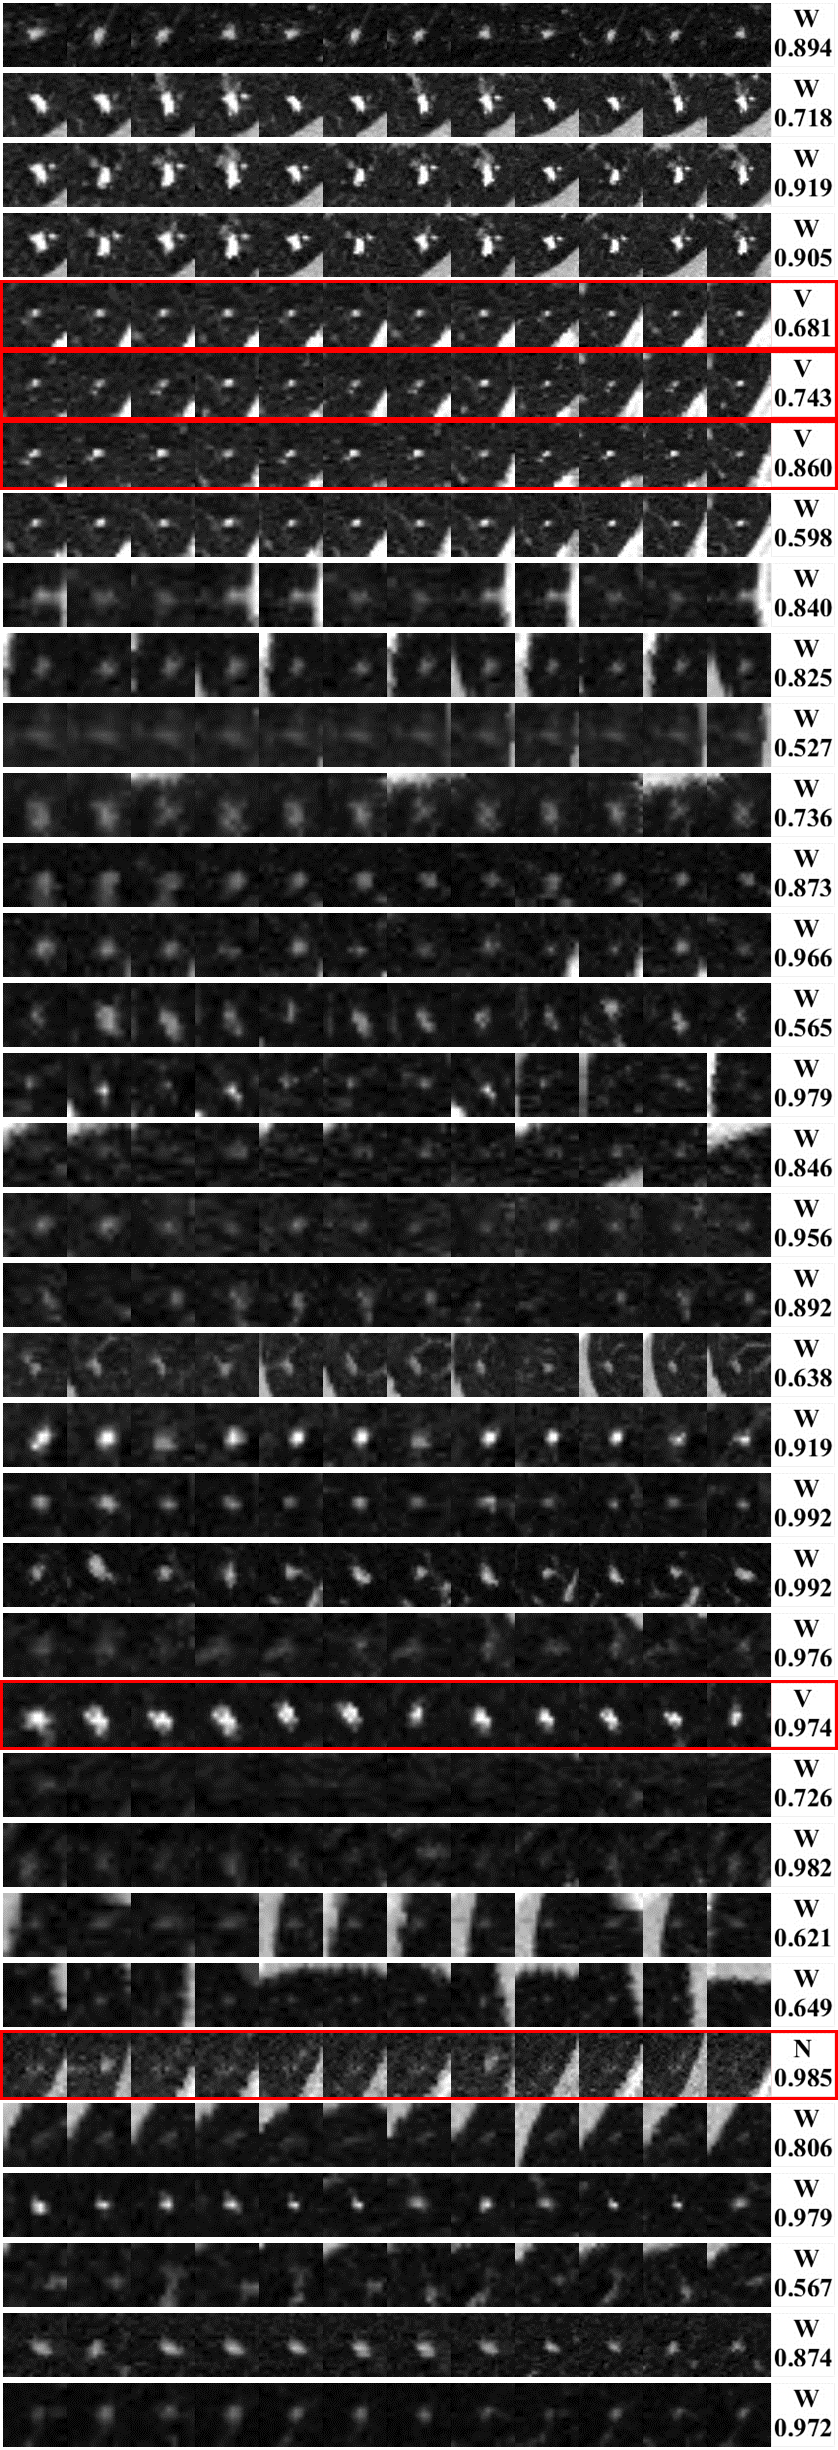
\includegraphics[width=0.45\columnwidth]{./images/elcap-msnodules-iso0}
}
\hspace{.1in}
\subfigure{
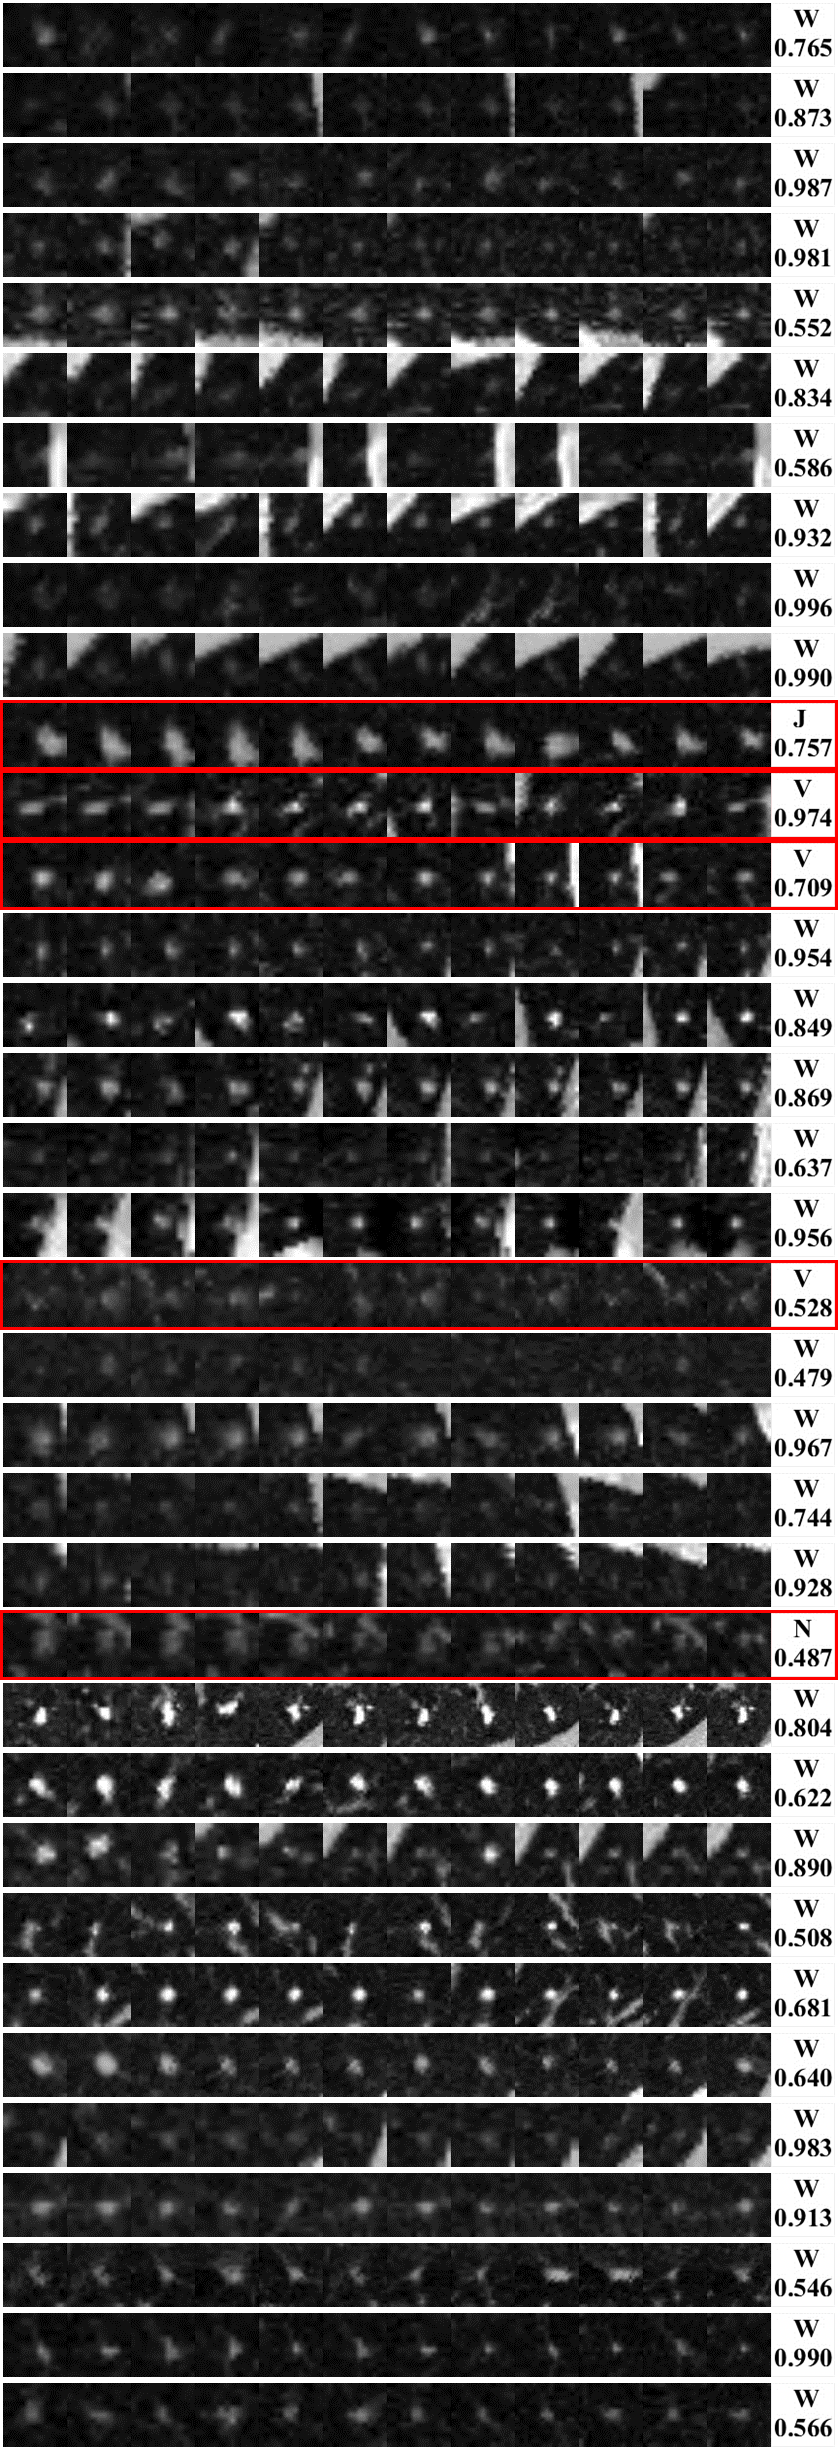
\includegraphics[width=0.45\columnwidth]{./images/elcap-msnodules-iso1}
}
\end{figure}

\newpage
\begin{figure}[H]
\centering
\subfigure{
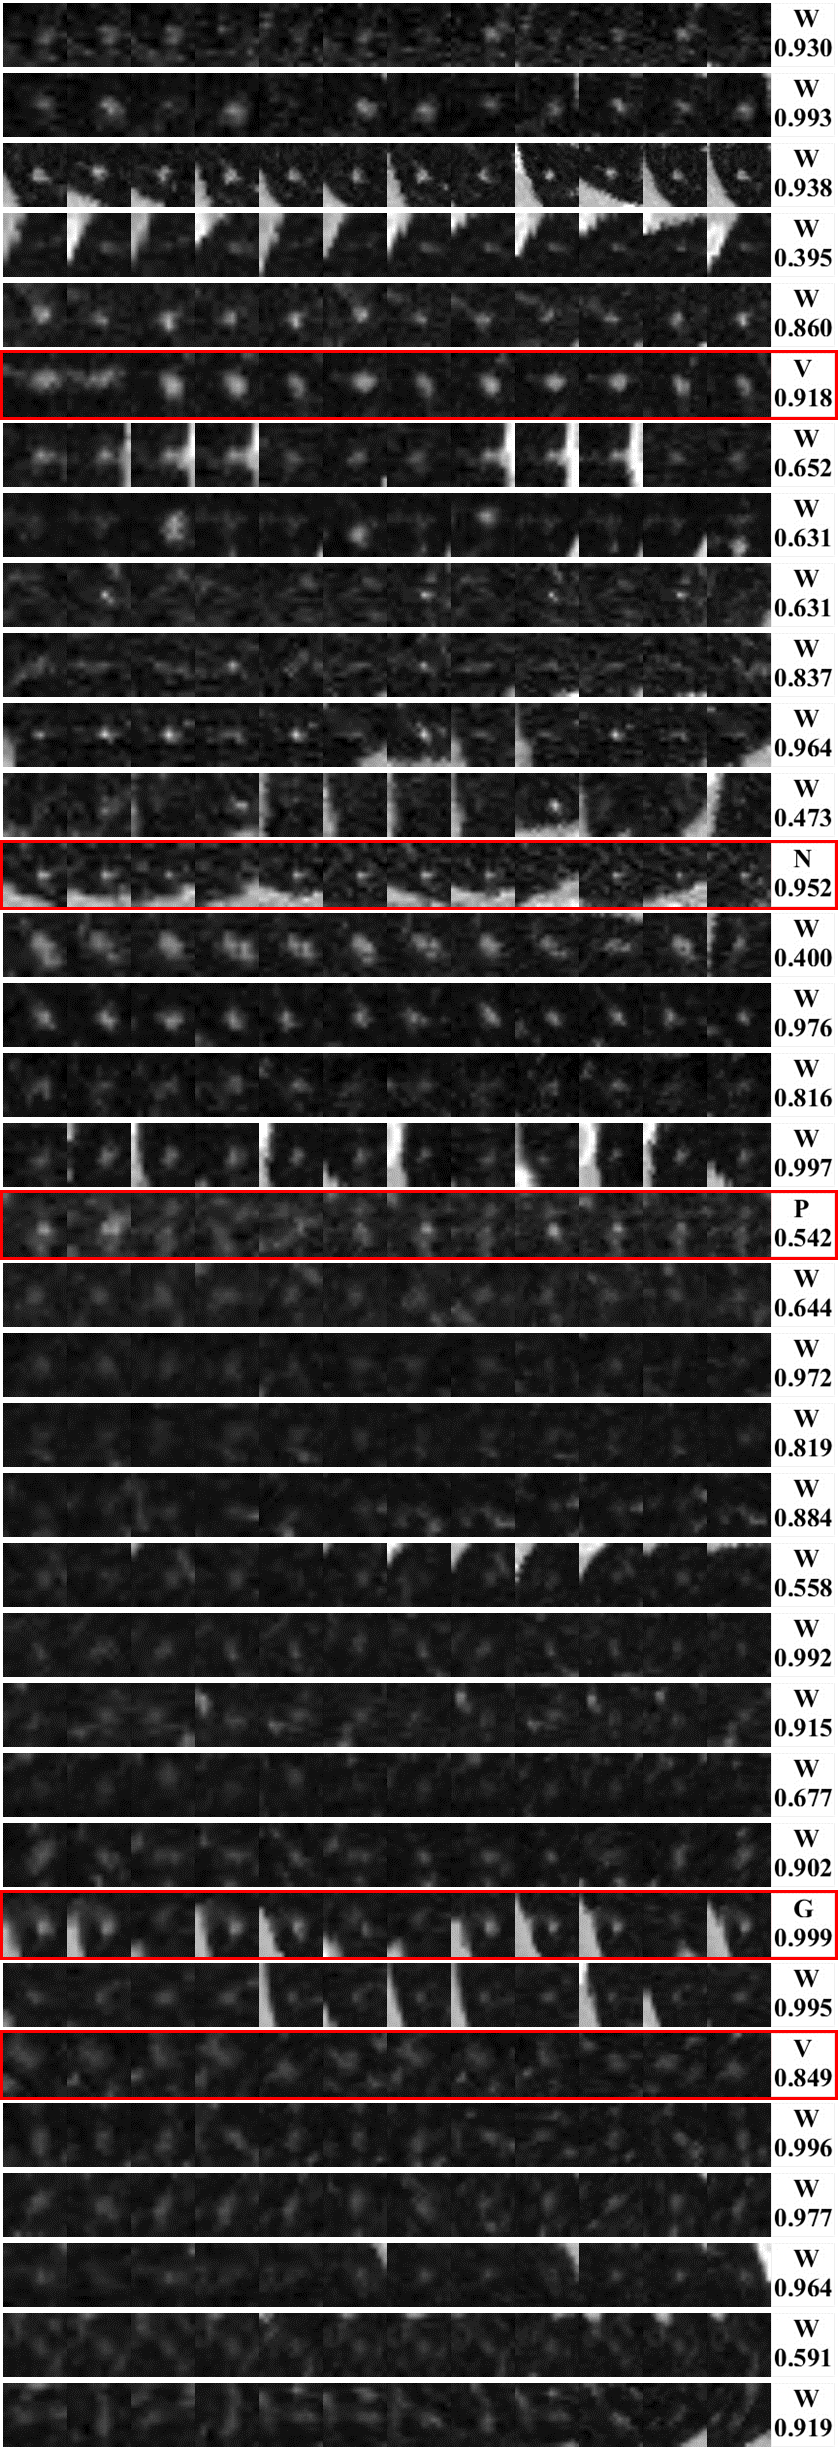
\includegraphics[width=0.45\columnwidth]{./images/elcap-msnodules-iso2}
}
\hspace{.1in}
\subfigure{
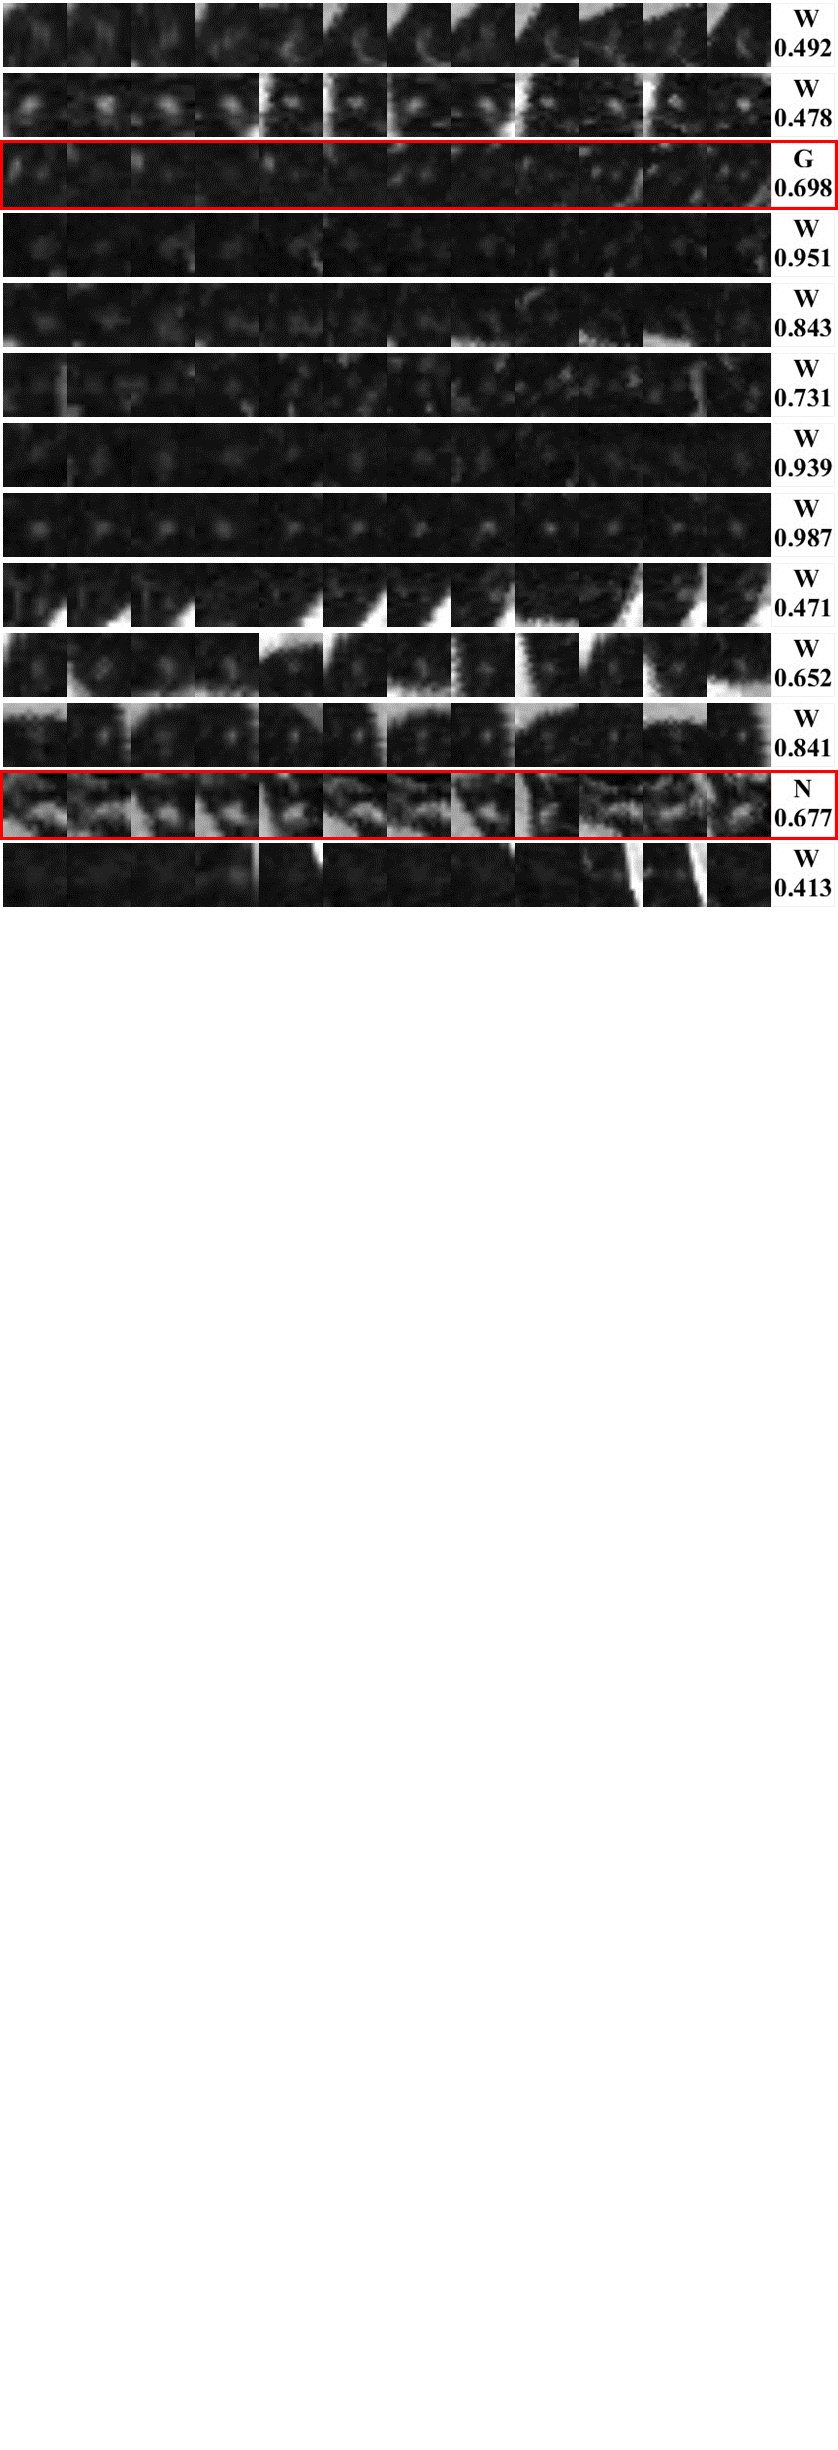
\includegraphics[width=0.45\columnwidth]{./images/elcap-msnodules-iso3}
}
\end{figure}

\newpage
\subsection{GGO for \emph{ms-nodules}}
\begin{figure}[H]
\centering
\subfigure{
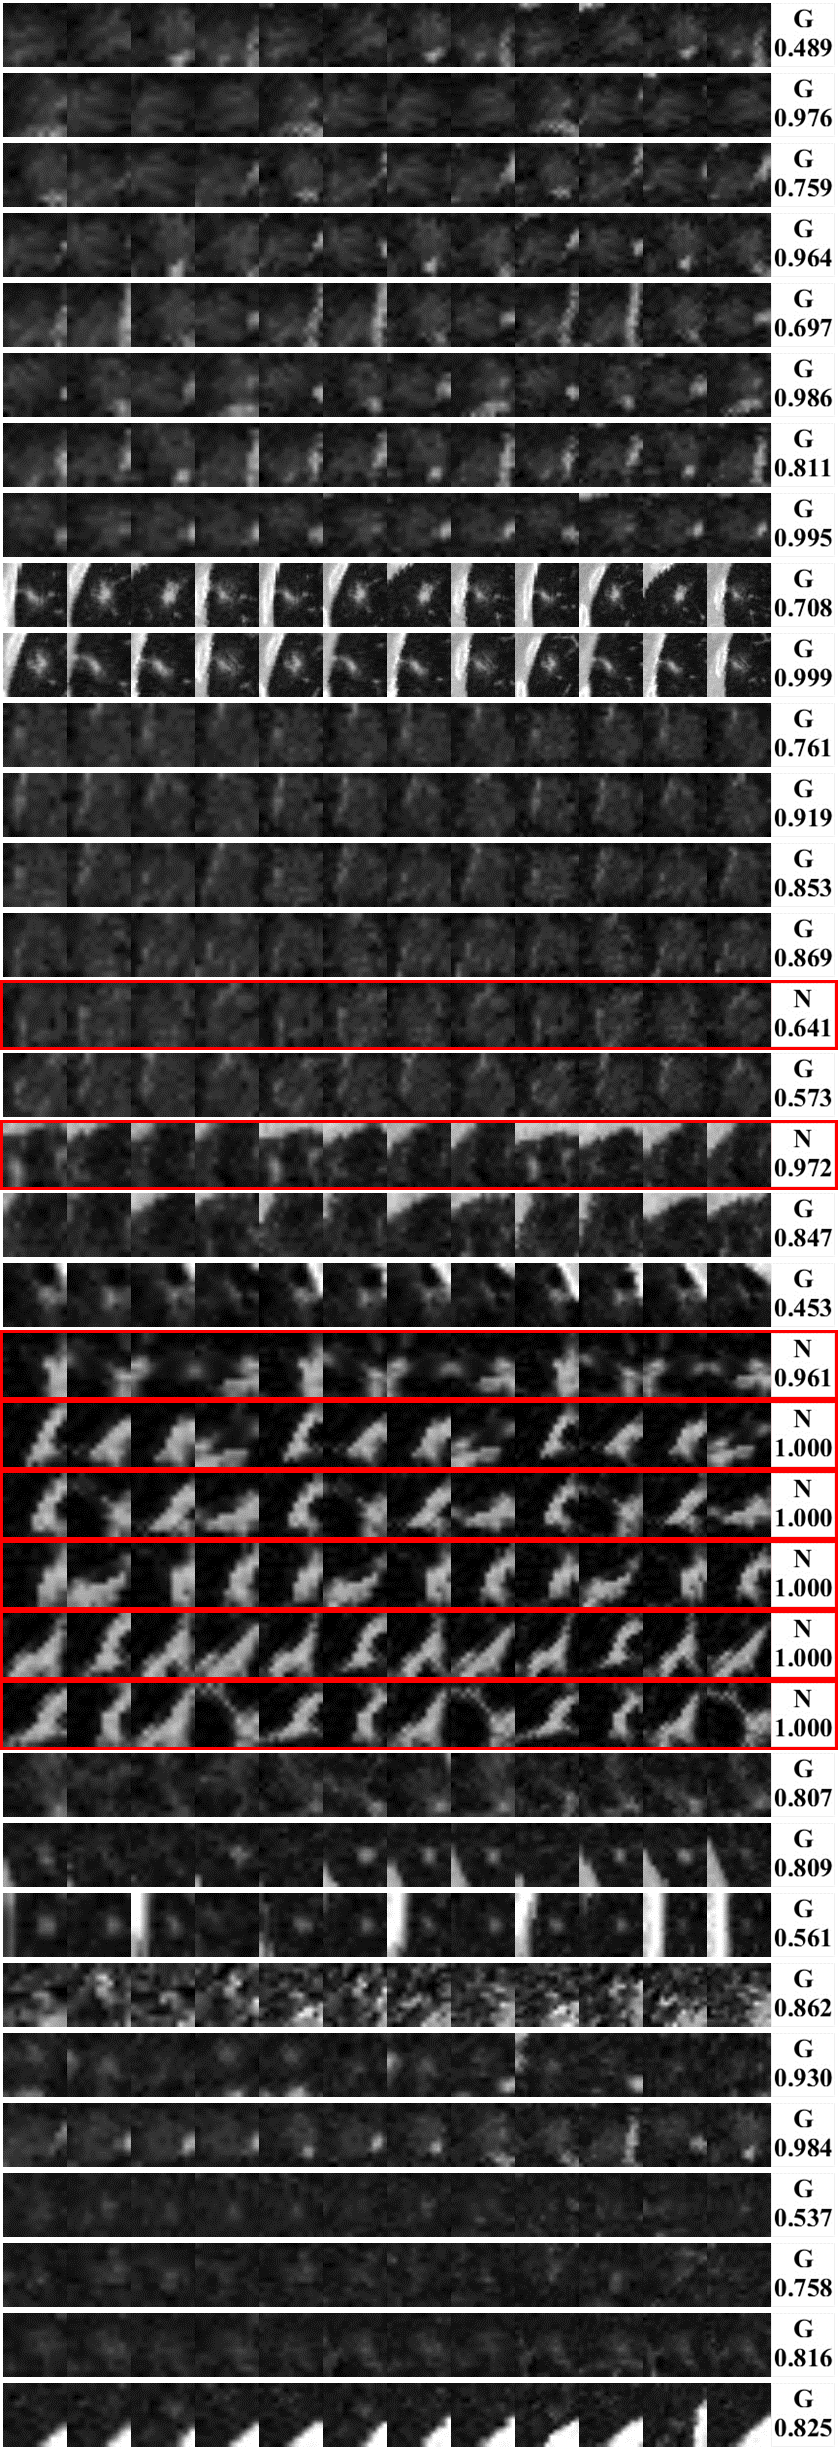
\includegraphics[width=0.45\columnwidth]{./images/elcap-msnodules-ggo0}
}
\hspace{.1in}
\subfigure{
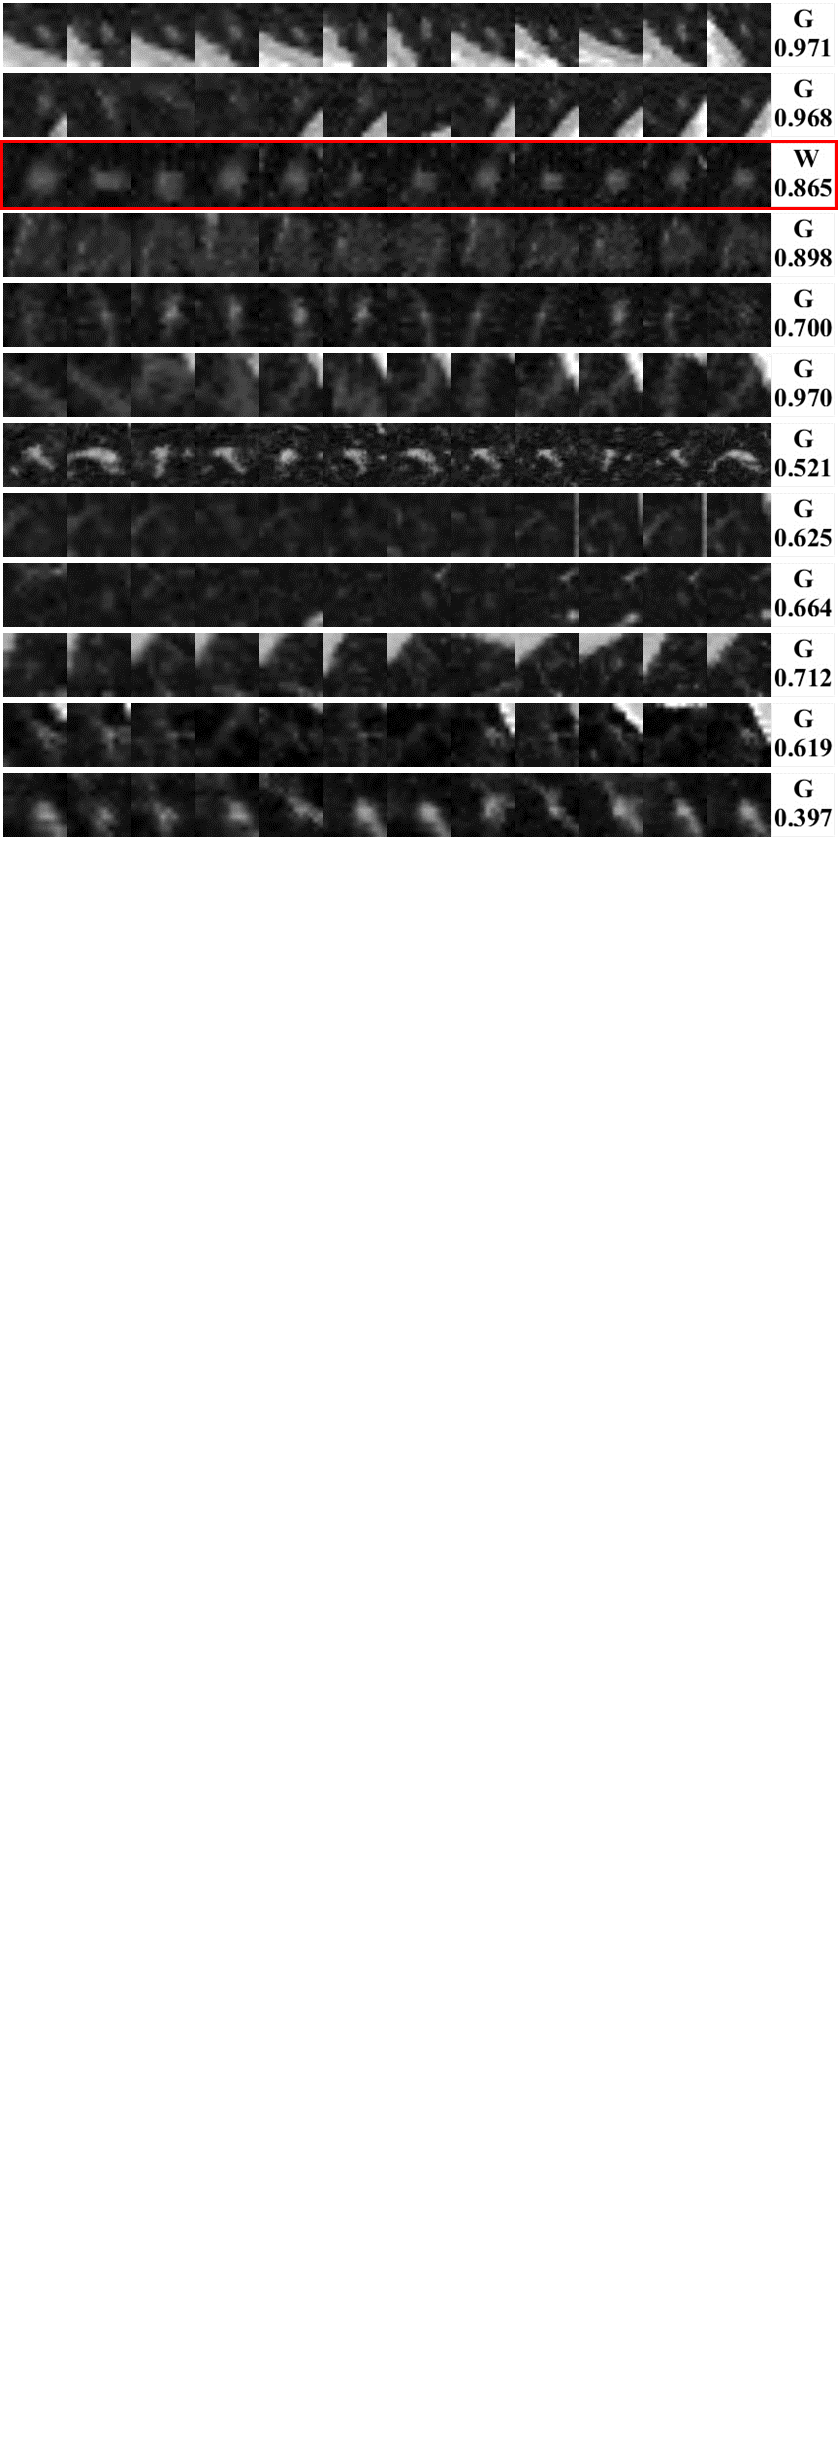
\includegraphics[width=0.45\columnwidth]{./images/elcap-msnodules-ggo1}
}
\end{figure}


\newpage
\subsection{Juxta-pleural for \emph{ms-nodules}}
\begin{figure}[H]
\centering
\subfigure{
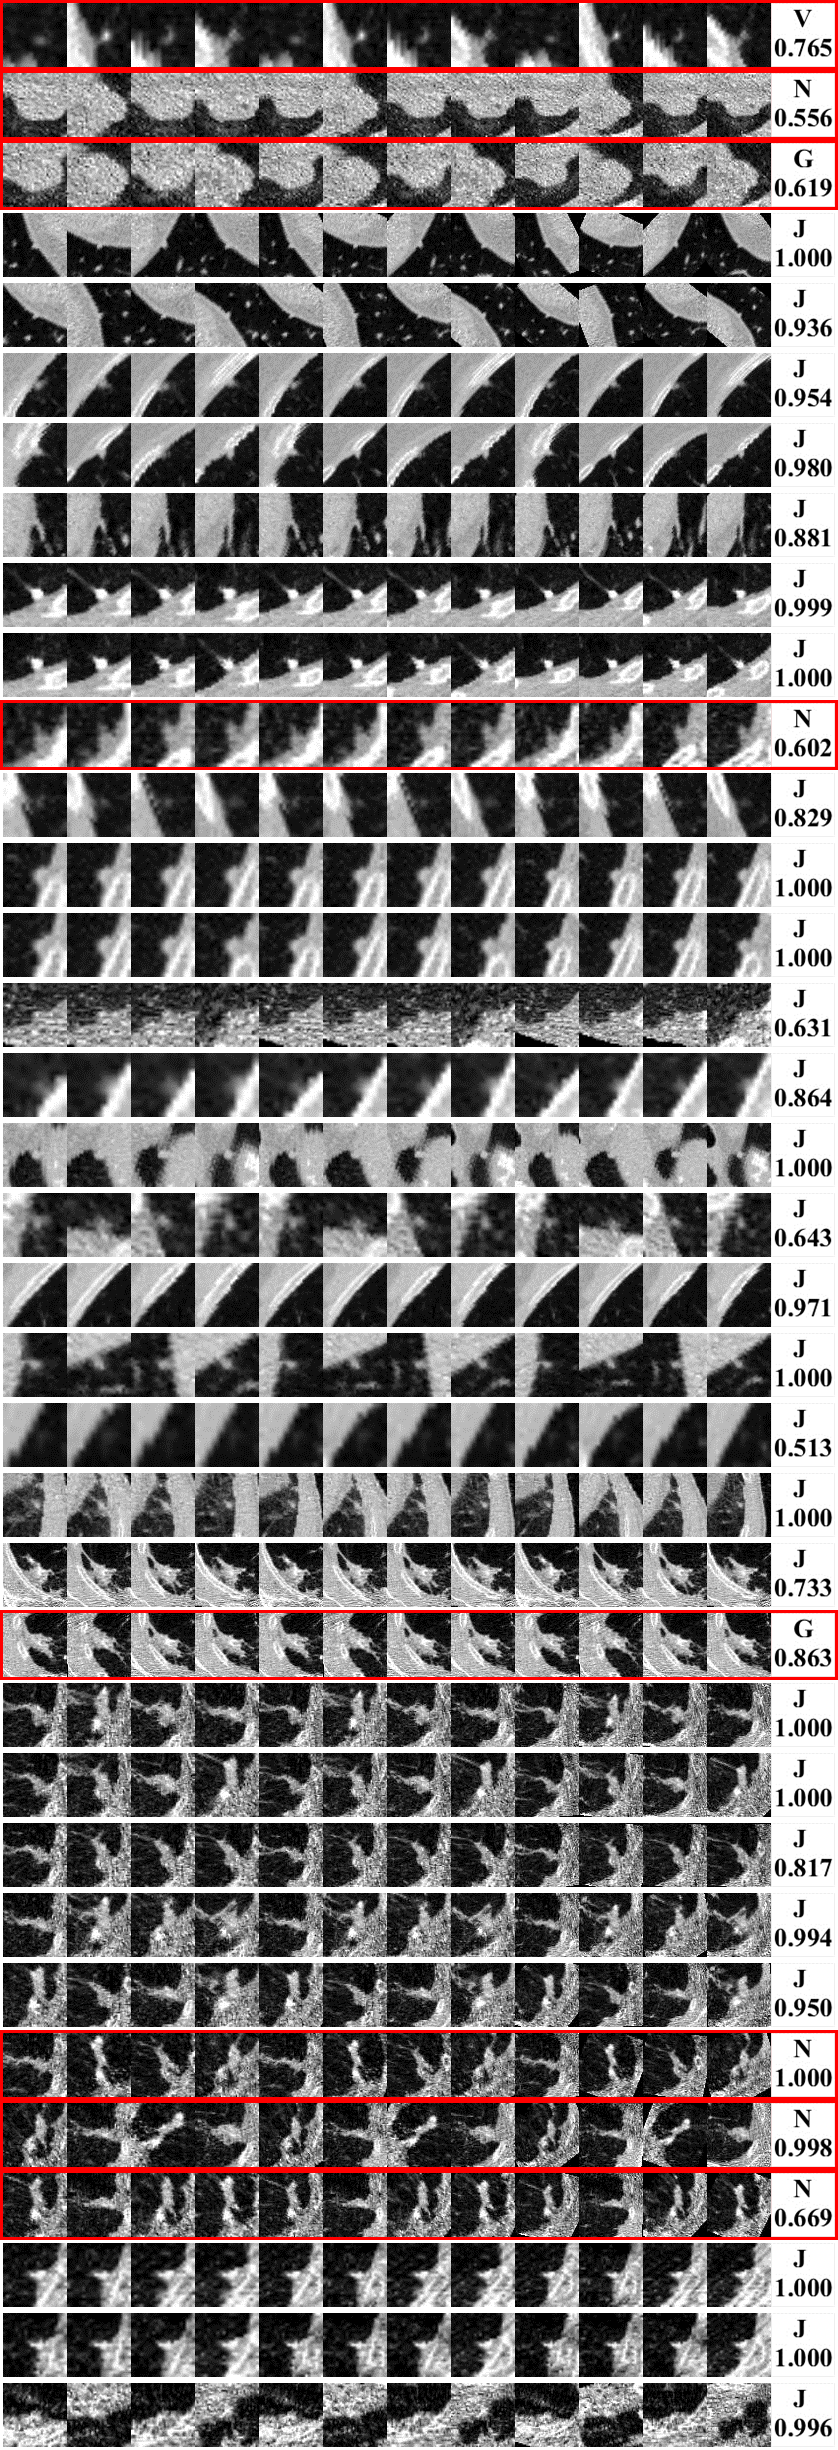
\includegraphics[width=0.45\columnwidth]{./images/elcap-msnodules-wall0}
}
\hspace{.1in}
\subfigure{
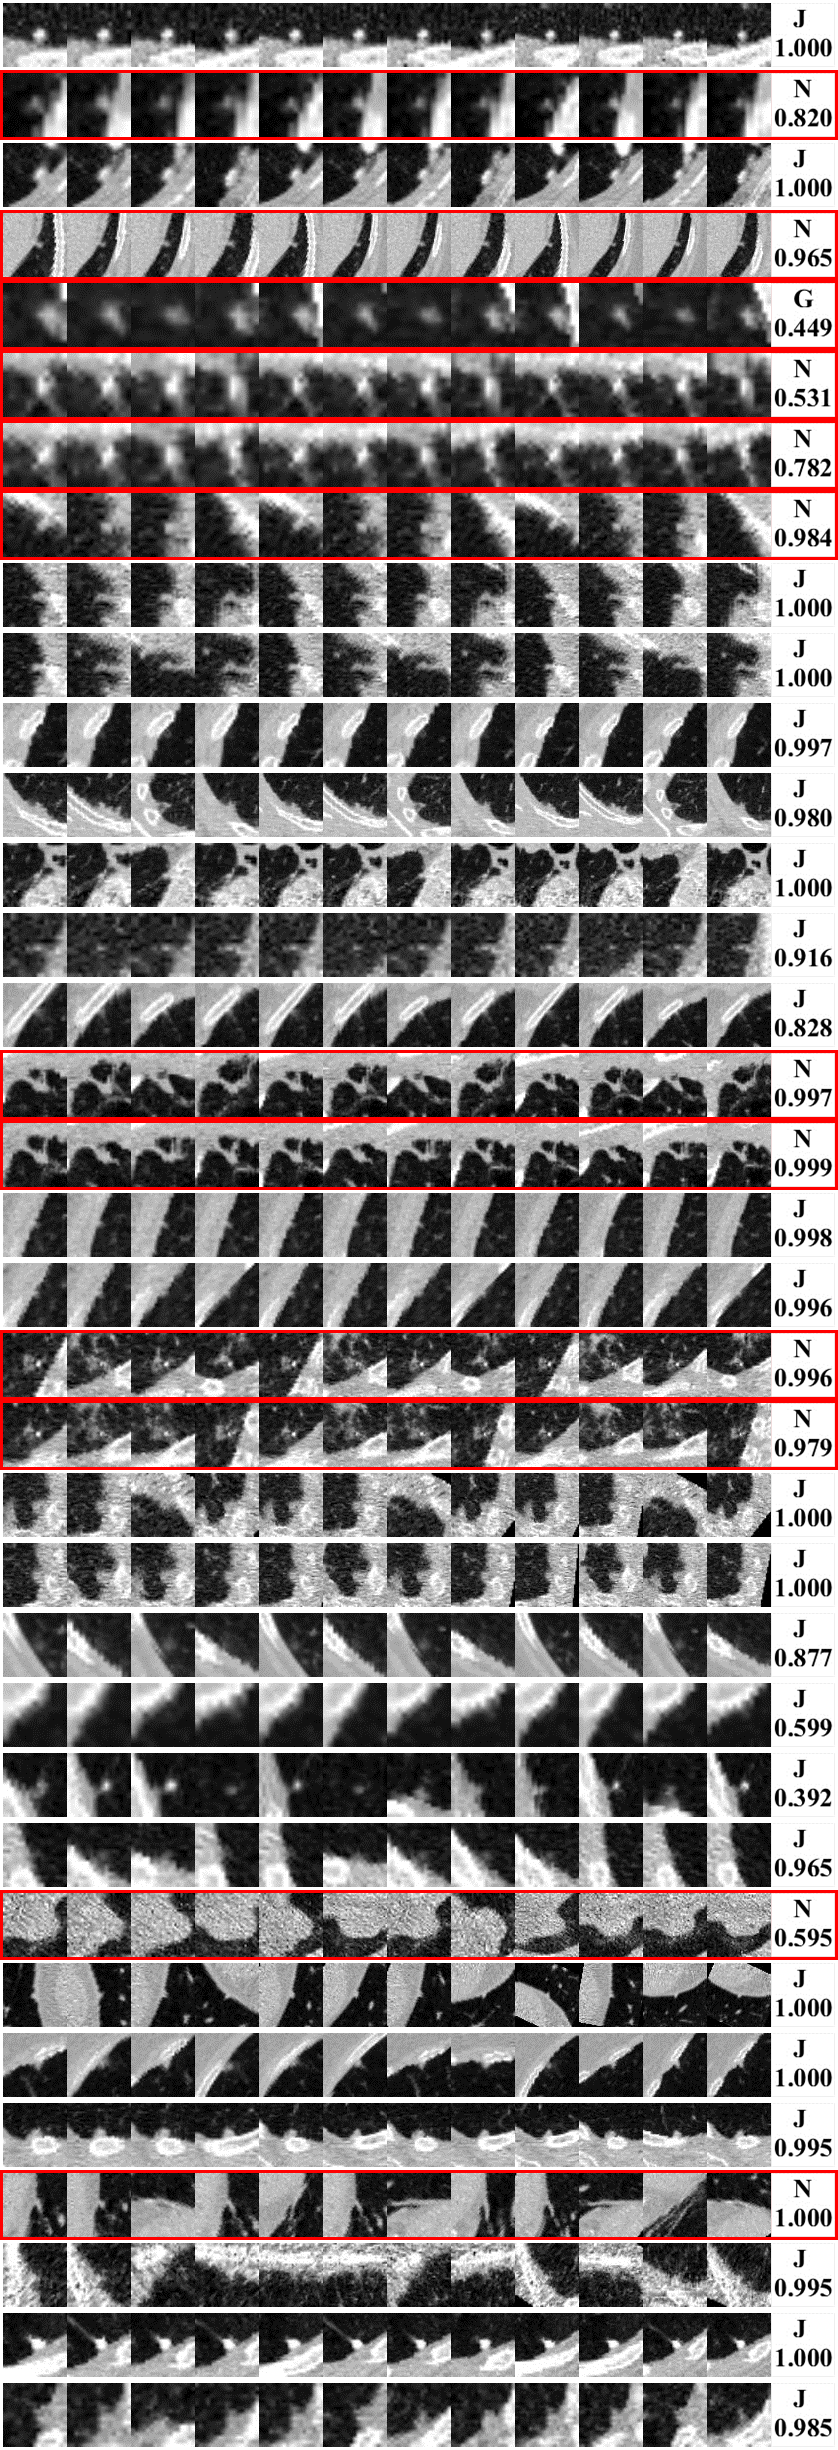
\includegraphics[width=0.45\columnwidth]{./images/elcap-msnodules-wall1}
}
\end{figure}
\newpage
\begin{figure}[H]
\centering
\subfigure{
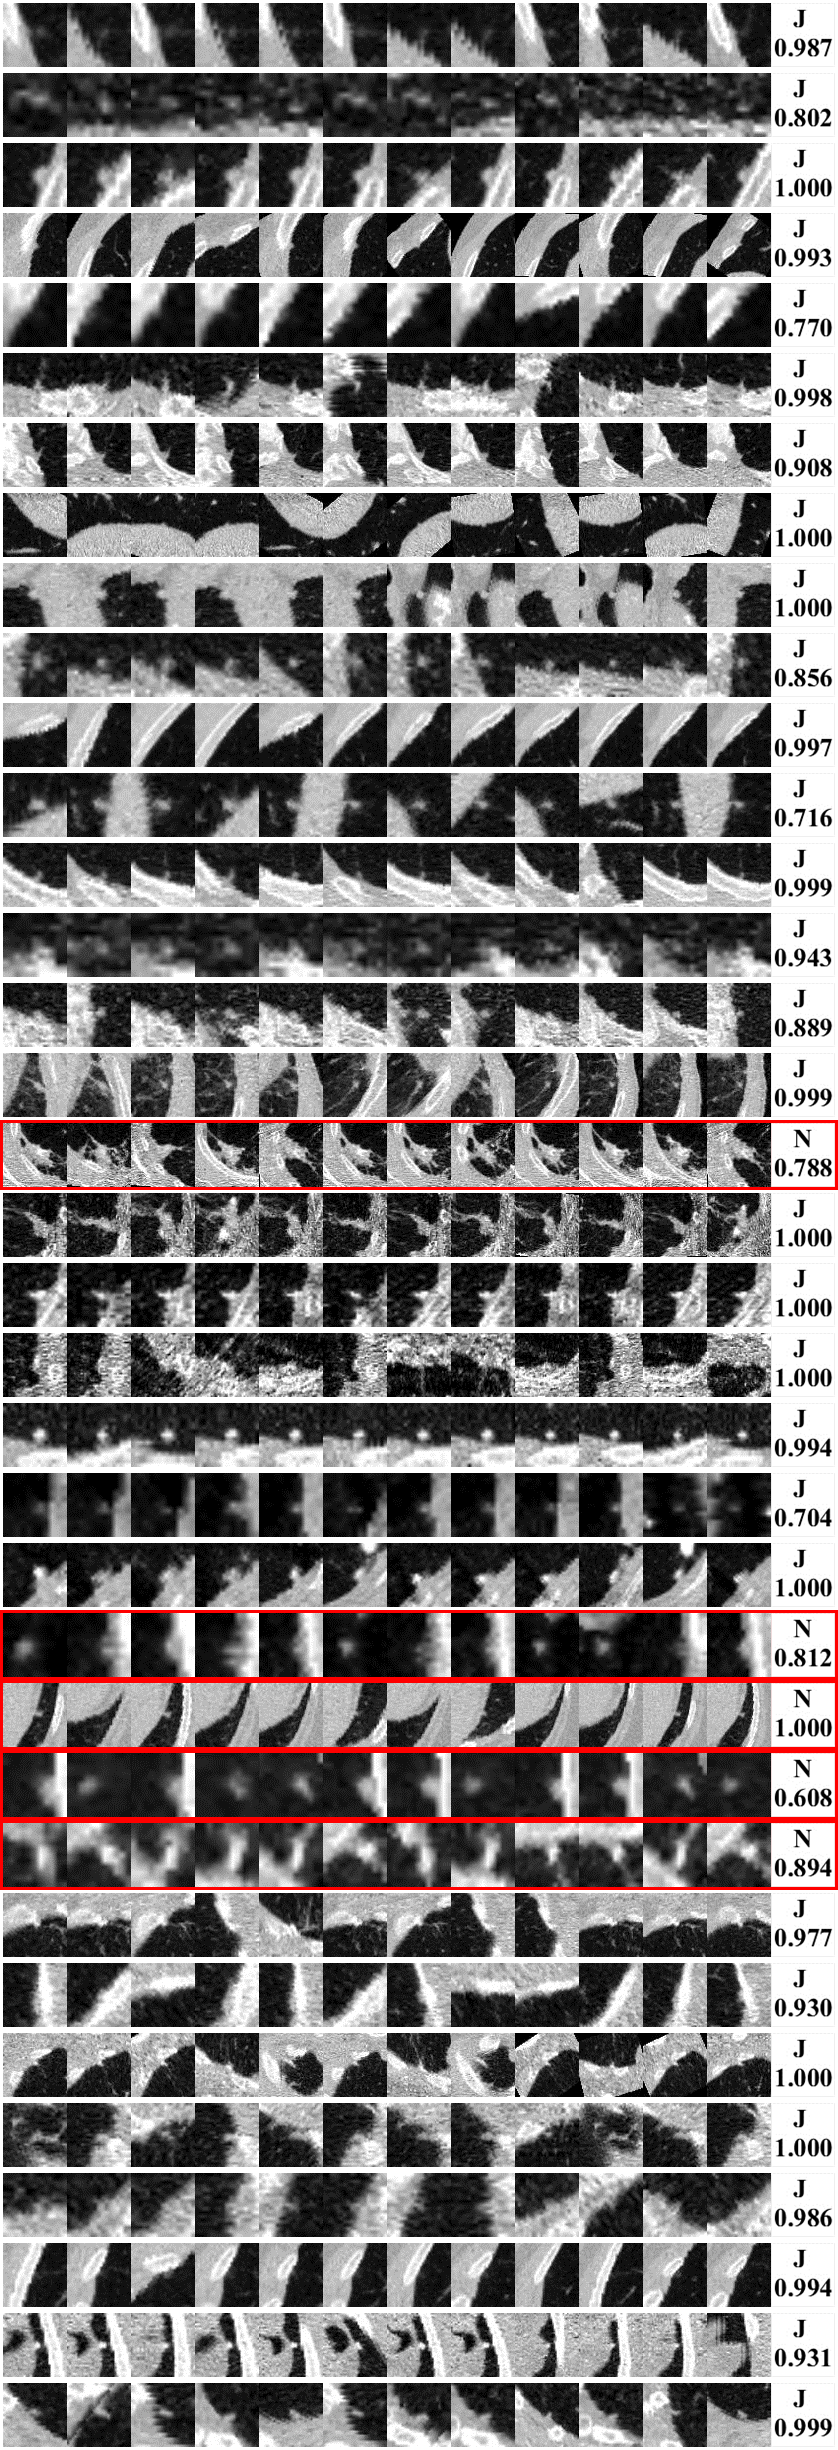
\includegraphics[width=0.45\columnwidth]{./images/elcap-msnodules-wall2}
}
\hspace{.1in}
\subfigure{
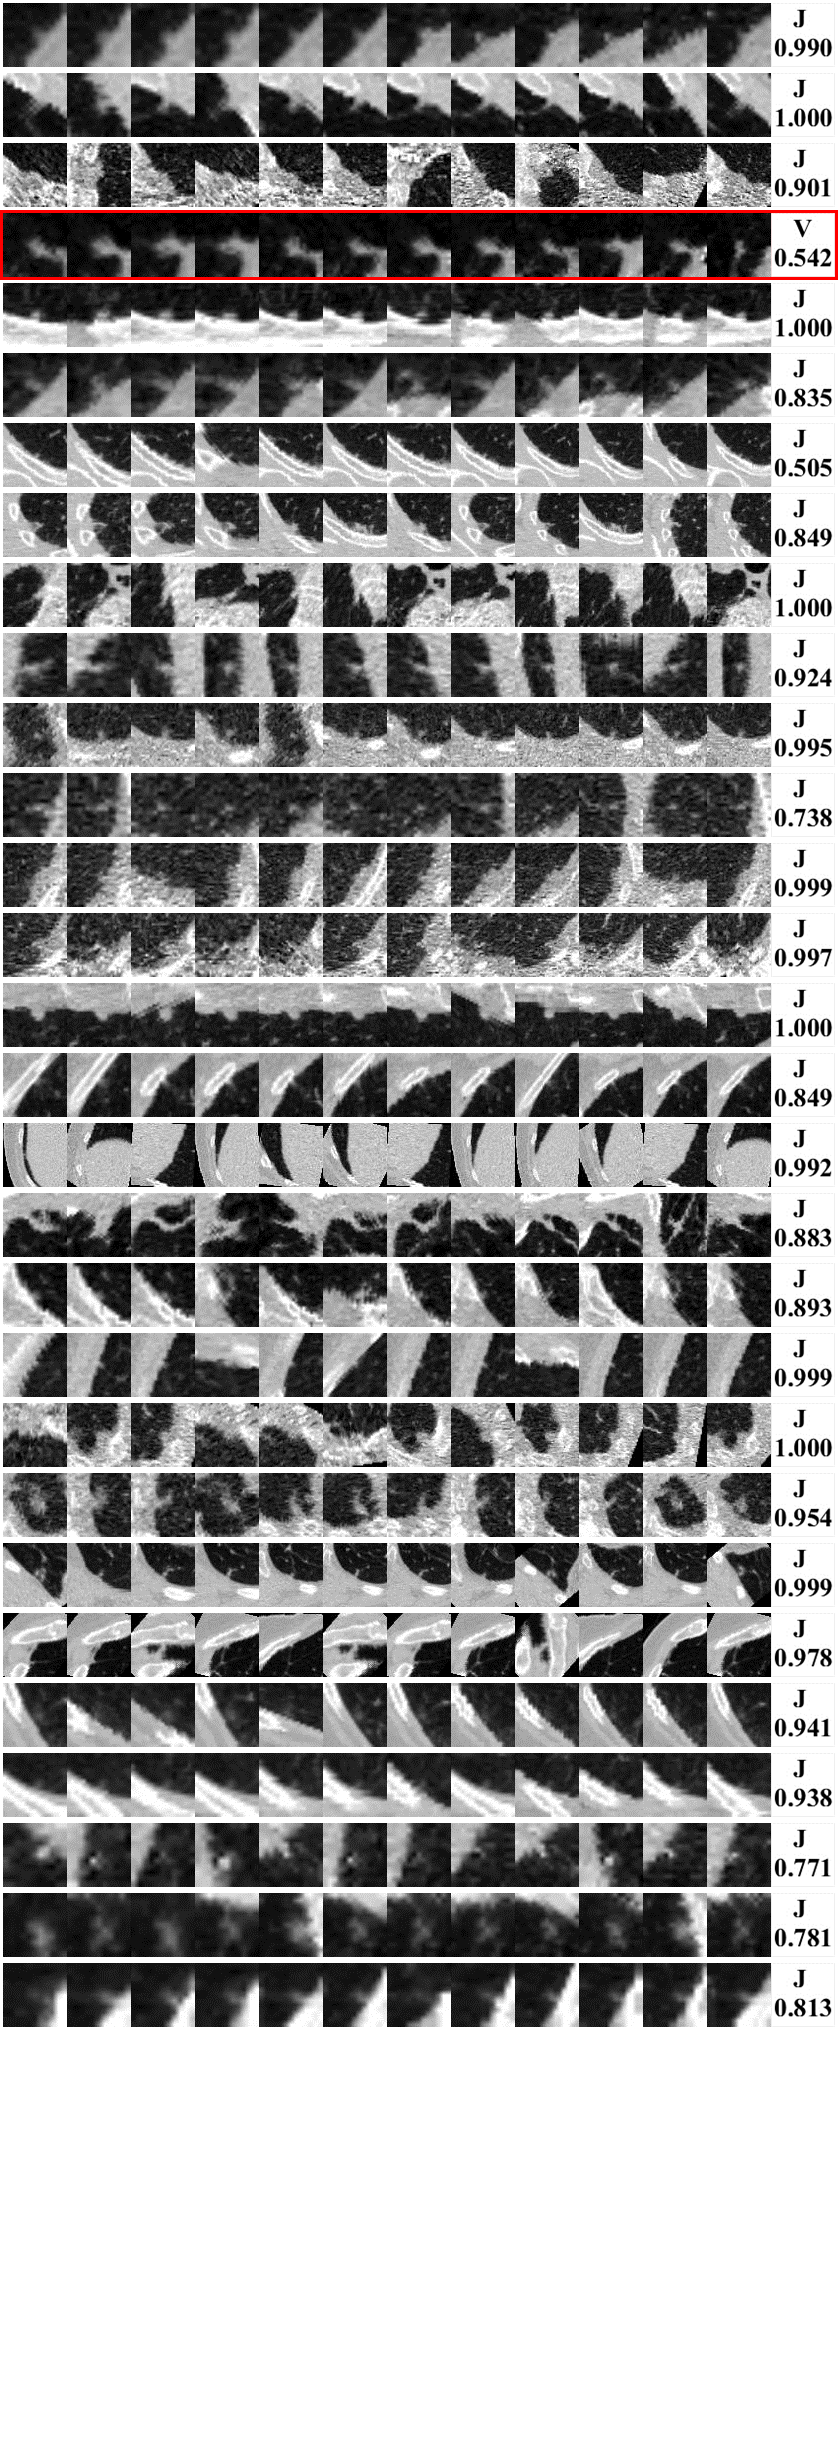
\includegraphics[width=0.45\columnwidth]{./images/elcap-msnodules-wall3}
}
\end{figure}

\newpage
\subsection{Pleural-tail for \emph{ms-nodules}}
\begin{figure}[H]
\centering
\subfigure{
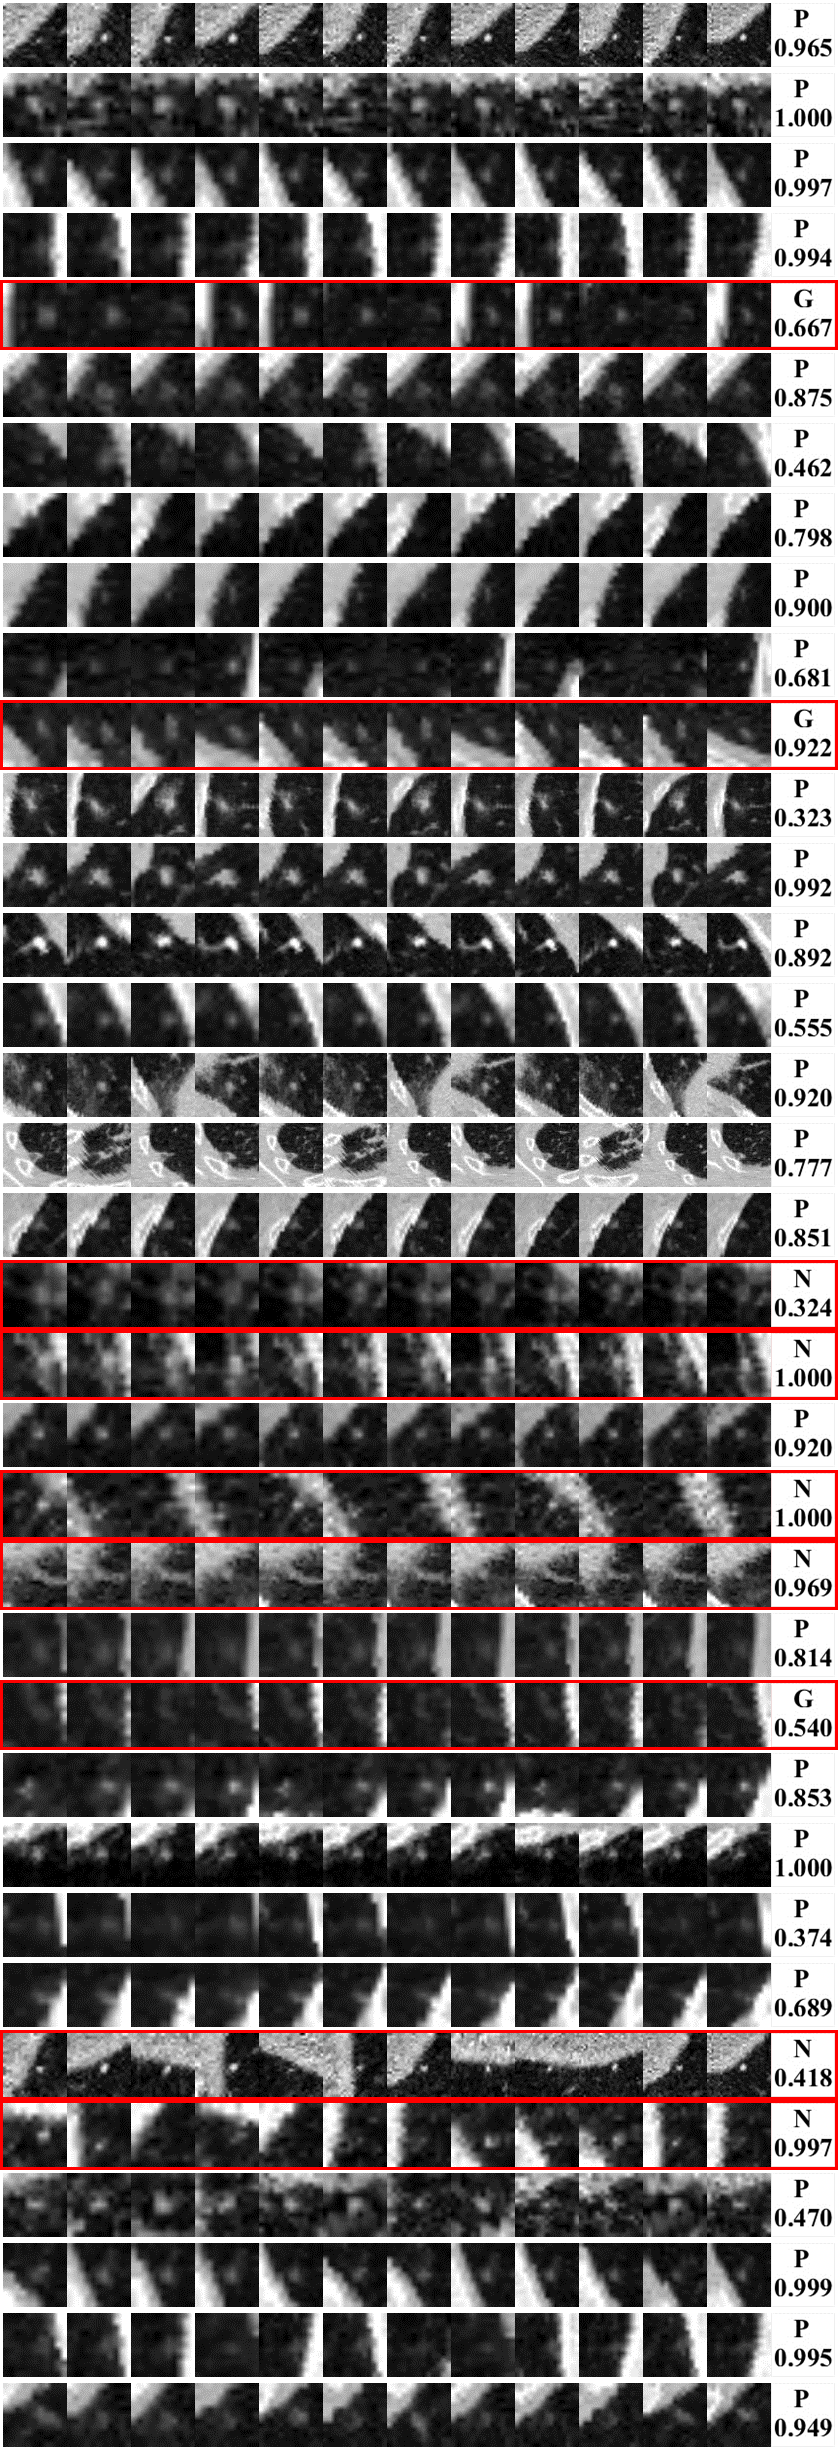
\includegraphics[width=0.45\columnwidth]{./images/elcap-msnodules-tail0}
}
\hspace{.1in}
\subfigure{
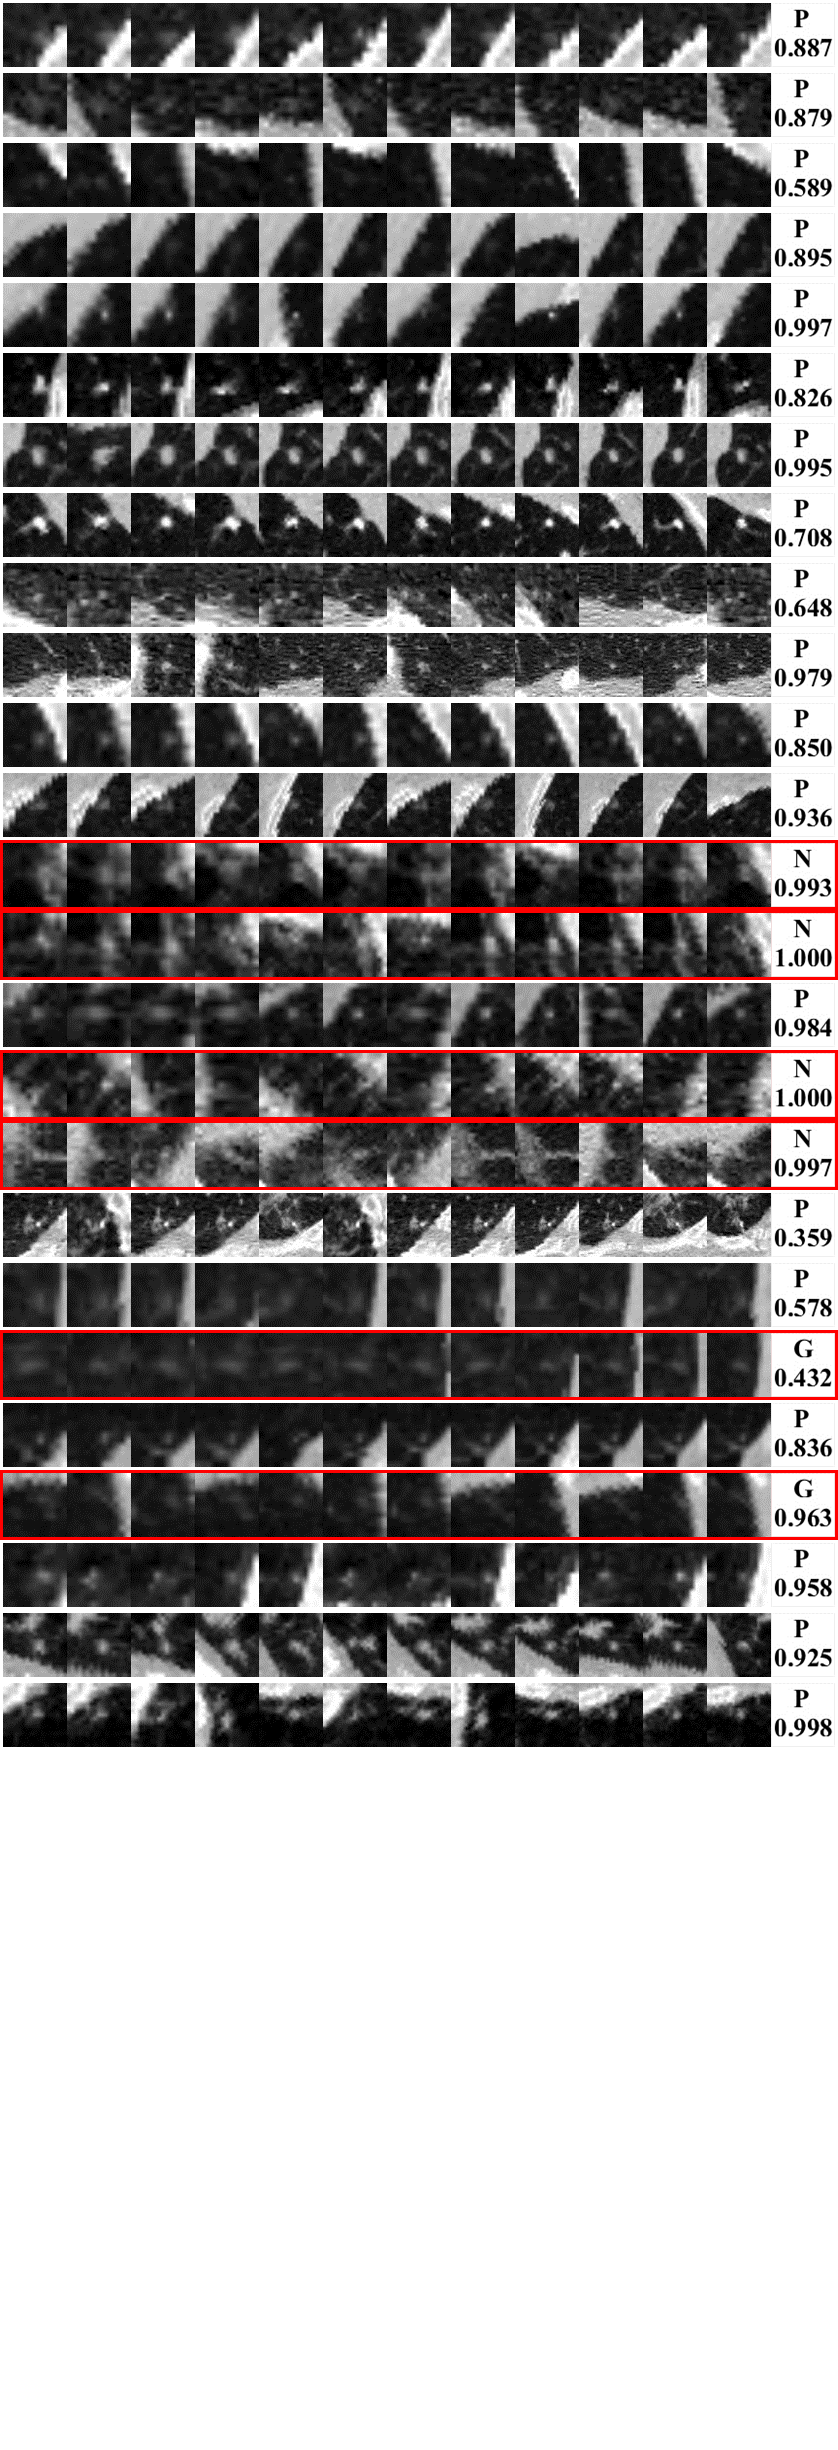
\includegraphics[width=0.45\columnwidth]{./images/elcap-msnodules-tail1}
}
\end{figure}

\newpage
\subsection{Vascularized for \emph{ms-nodules}}
\begin{figure}[H]
\centering
\subfigure{
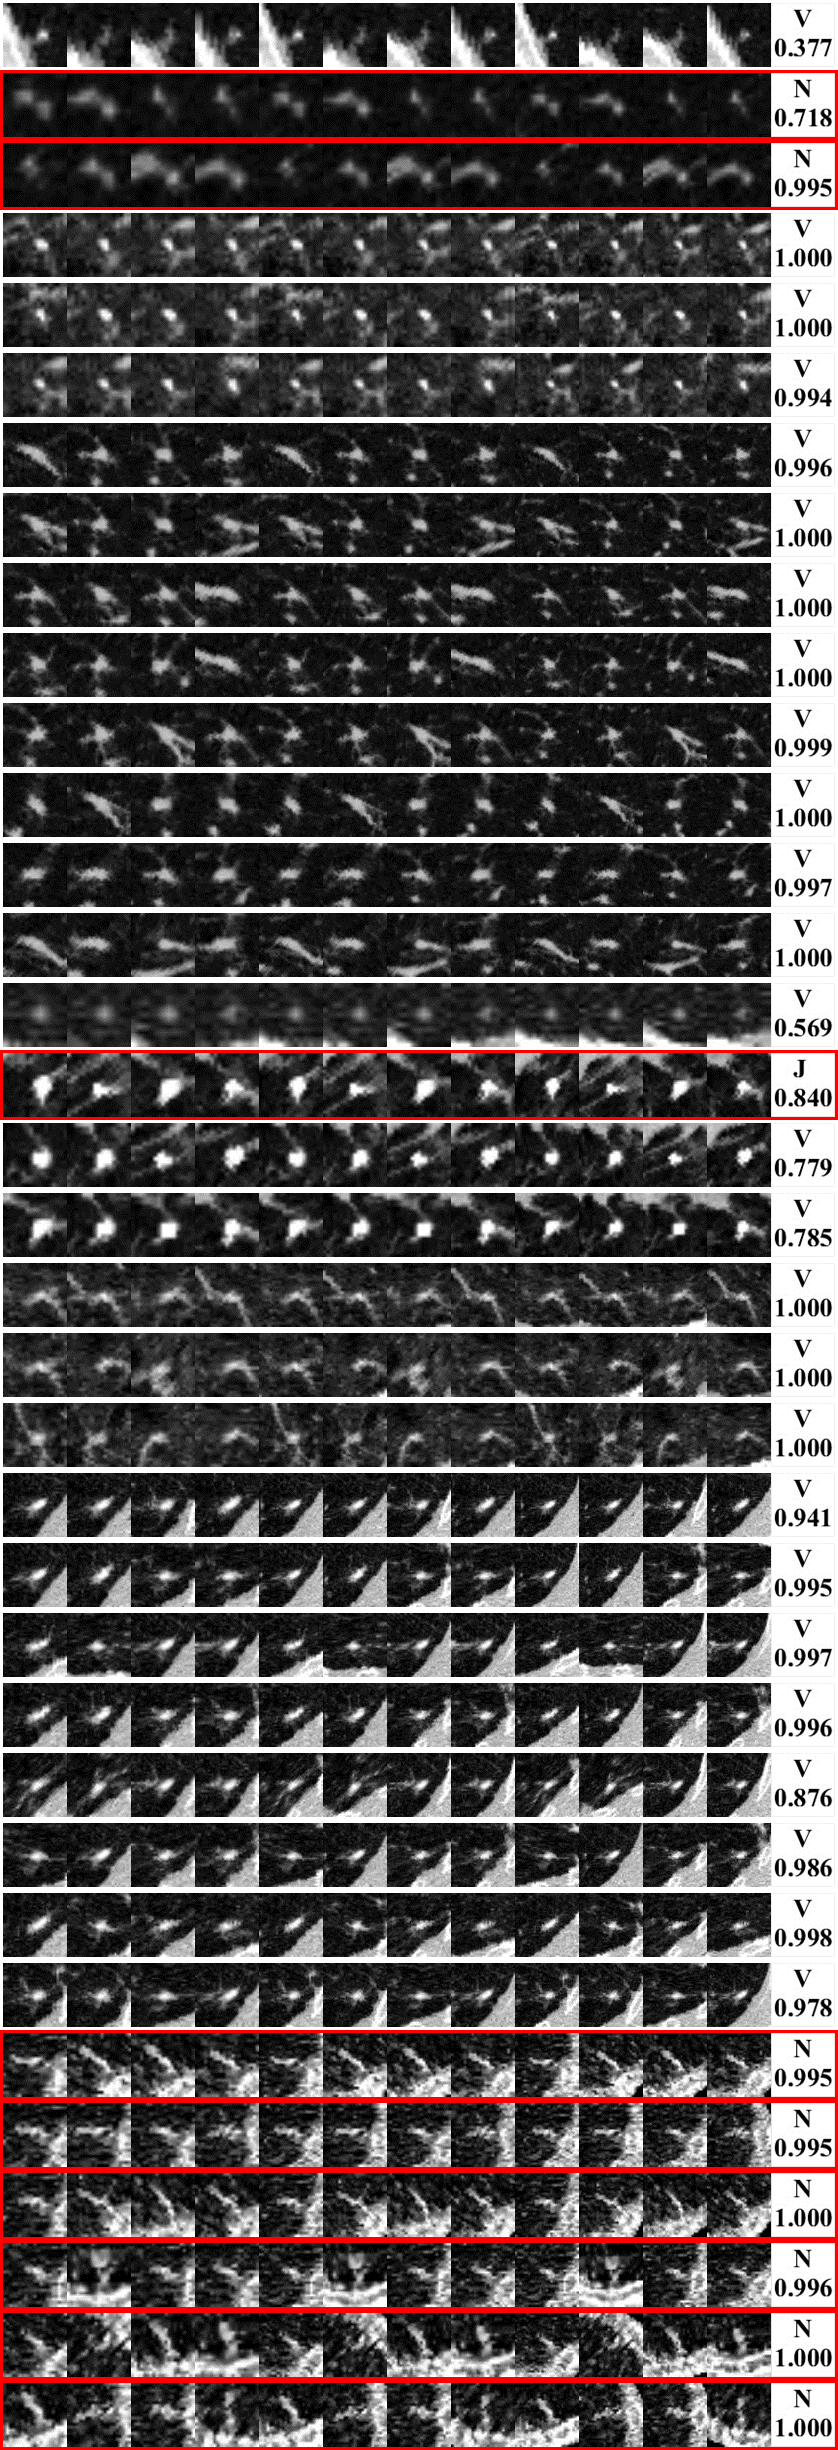
\includegraphics[width=0.45\columnwidth]{./images/elcap-msnodules-vessel0}
}
\hspace{.1in}
\subfigure{
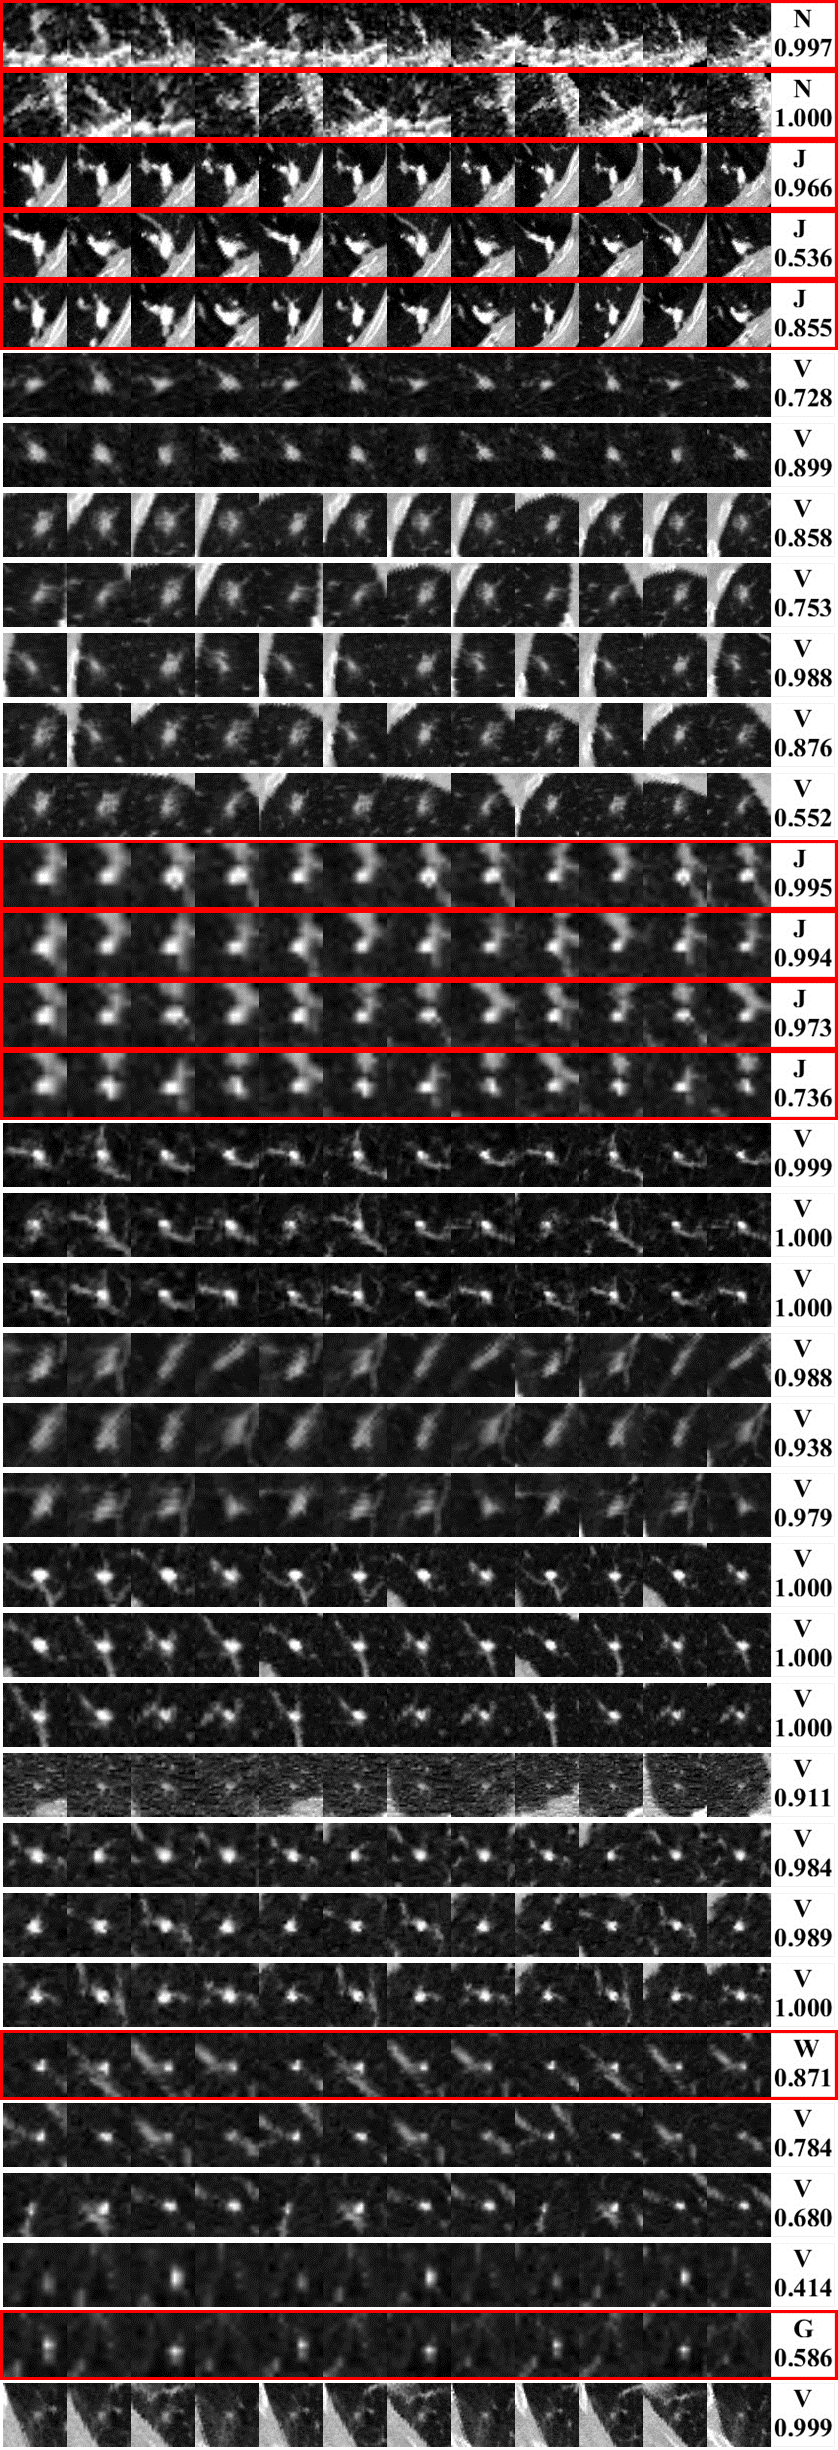
\includegraphics[width=0.45\columnwidth]{./images/elcap-msnodules-vessel1}
}
\end{figure}
\newpage
\begin{figure}[H]
\centering
\subfigure{
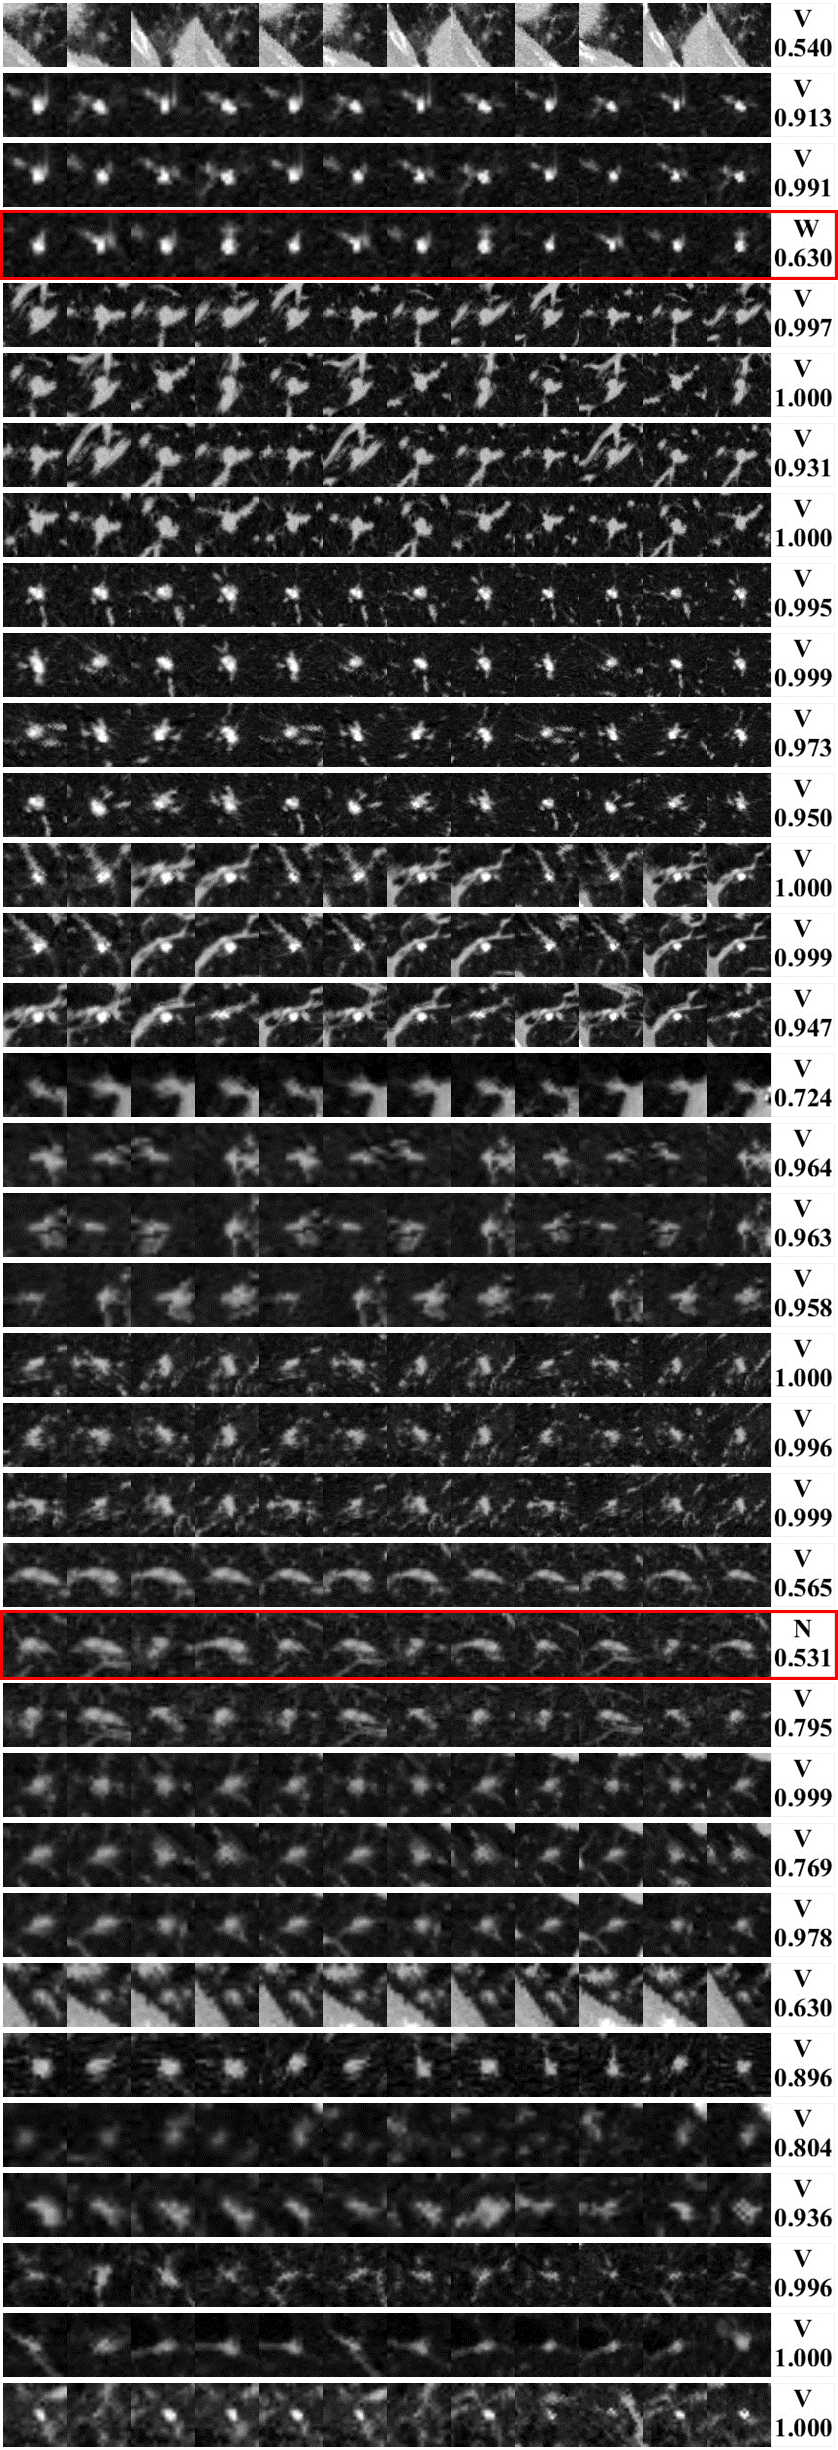
\includegraphics[width=0.45\columnwidth]{./images/elcap-msnodules-vessel2}
}
\hspace{.1in}
\subfigure{
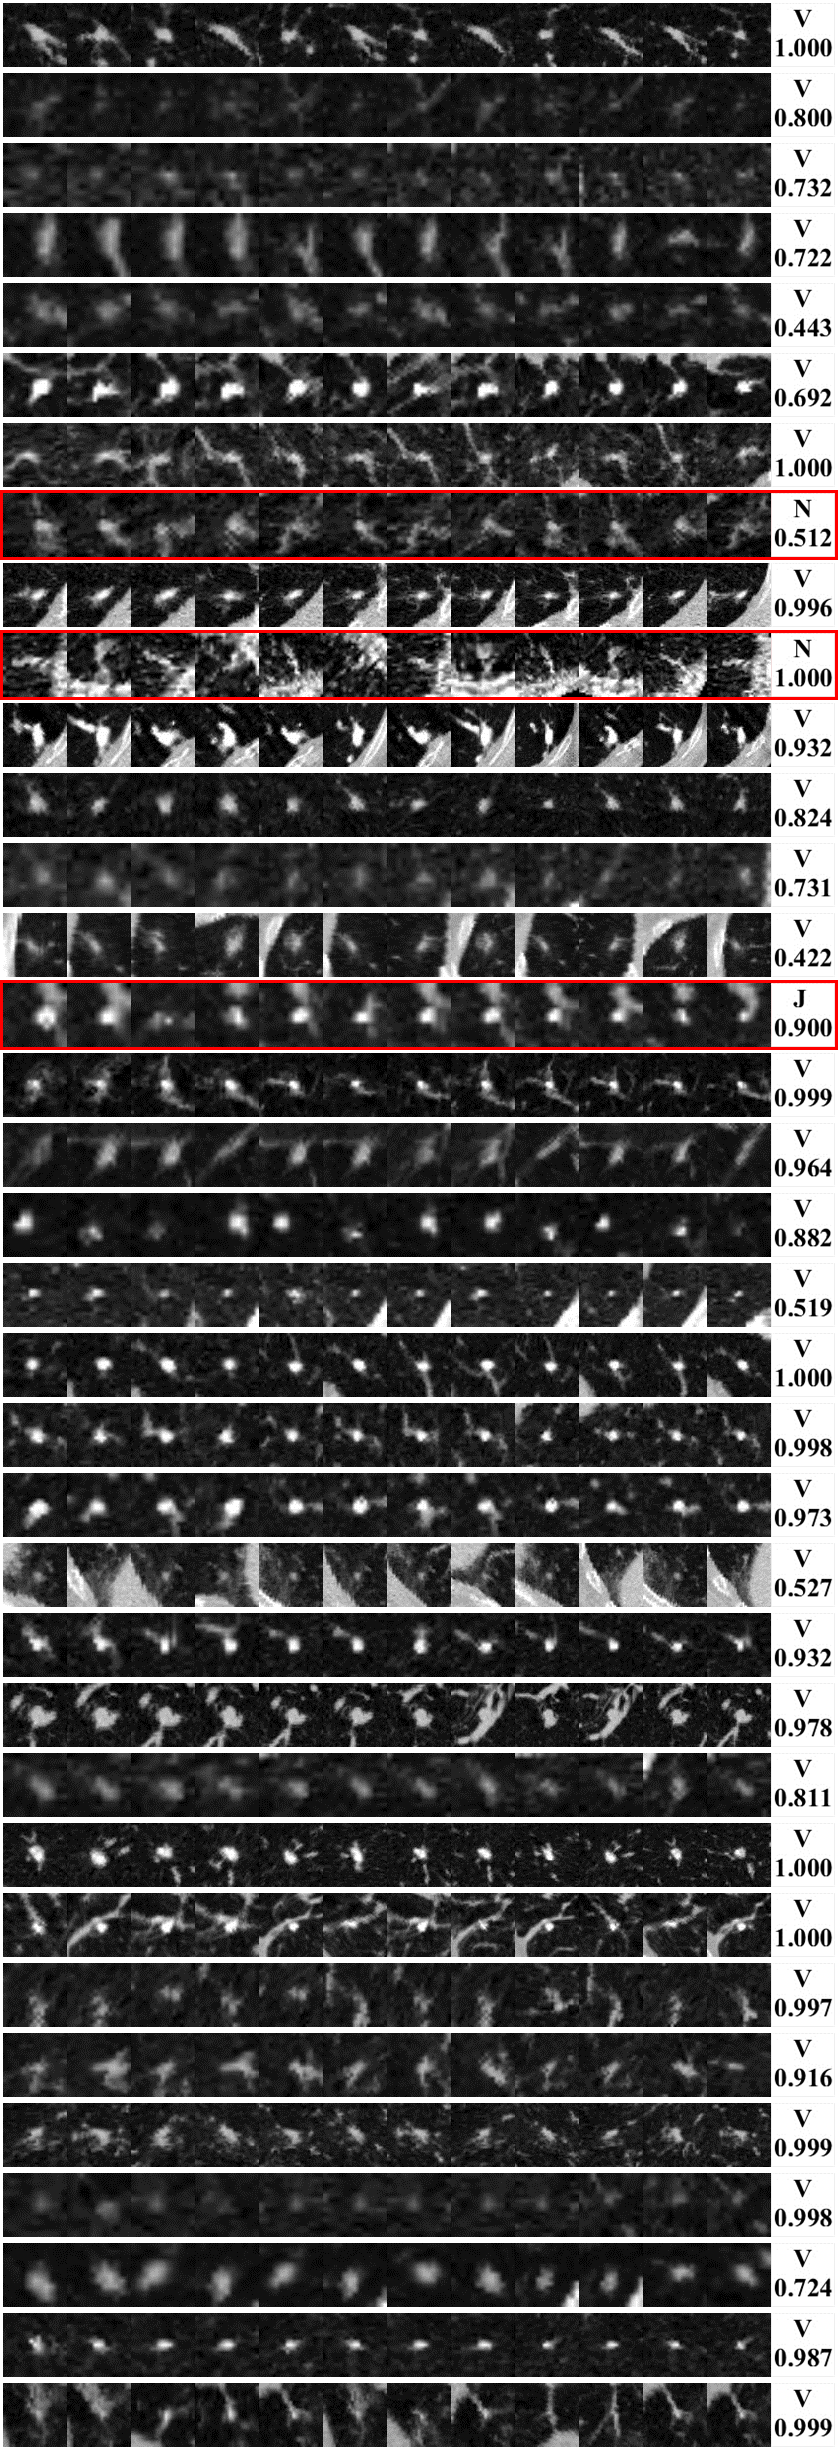
\includegraphics[width=0.45\columnwidth]{./images/elcap-msnodules-vessel3}
}
\end{figure}
\newpage
\begin{figure}[H]
\centering
\subfigure{
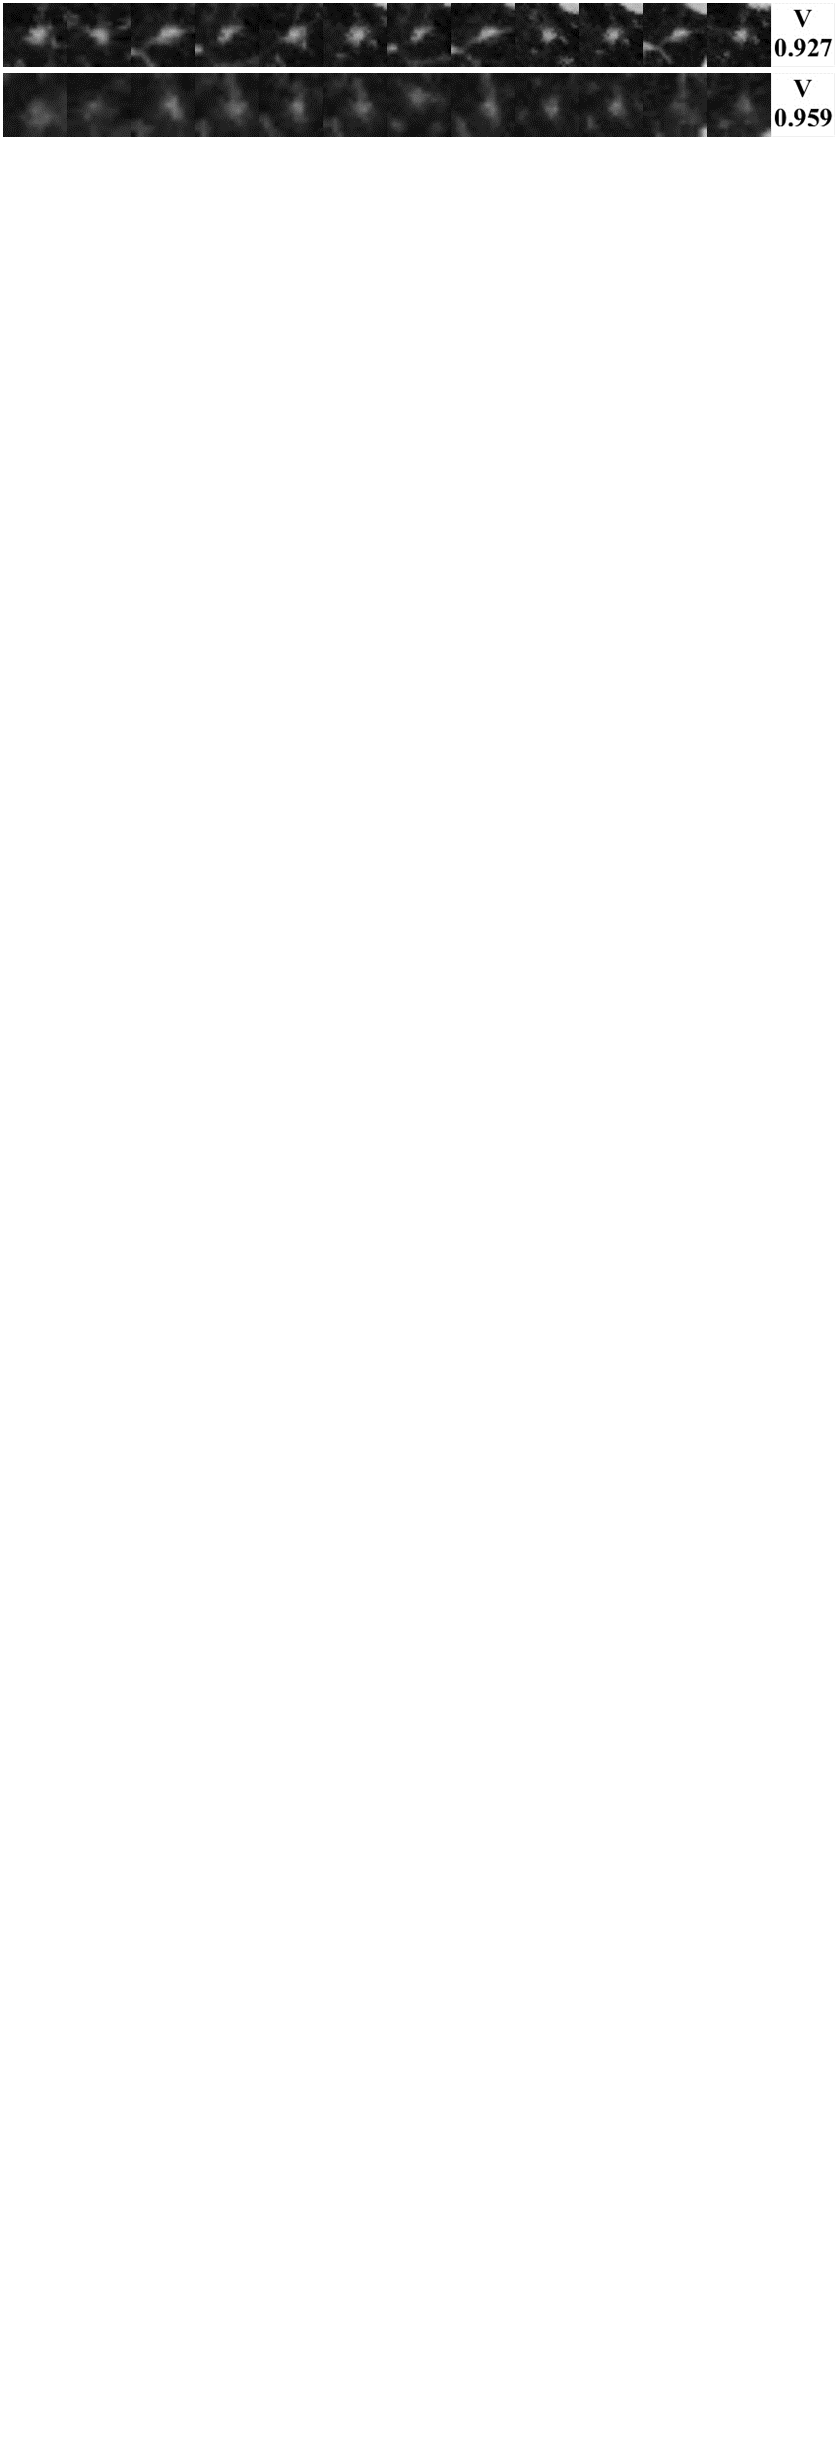
\includegraphics[width=0.45\columnwidth]{./images/elcap-msnodules-vessel4}
}
\end{figure}

\newpage
\subsection{NON-NODULE for \emph{ms-nodules}}
\begin{figure}[H]
\centering
\subfigure{
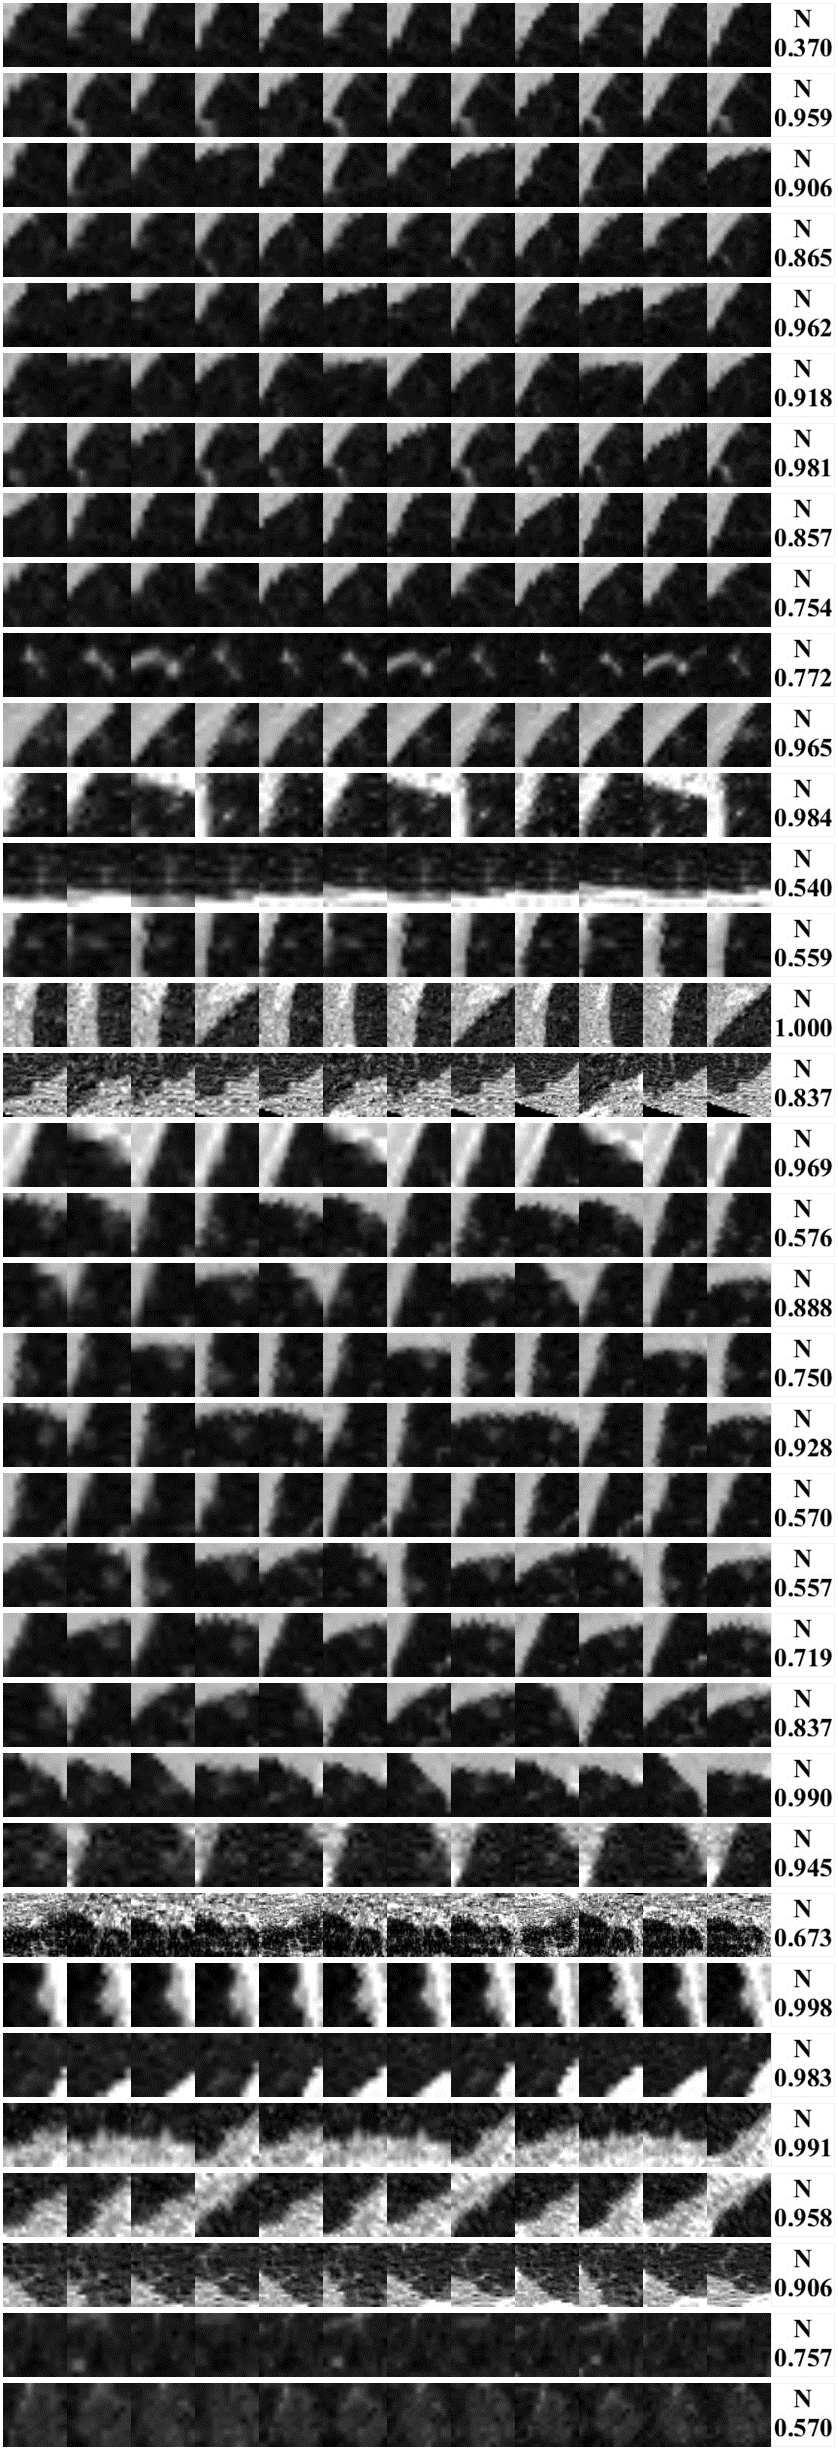
\includegraphics[width=0.45\columnwidth]{./images/elcap-msnodules-nonnodule0}
}
\hspace{.1in}
\subfigure{
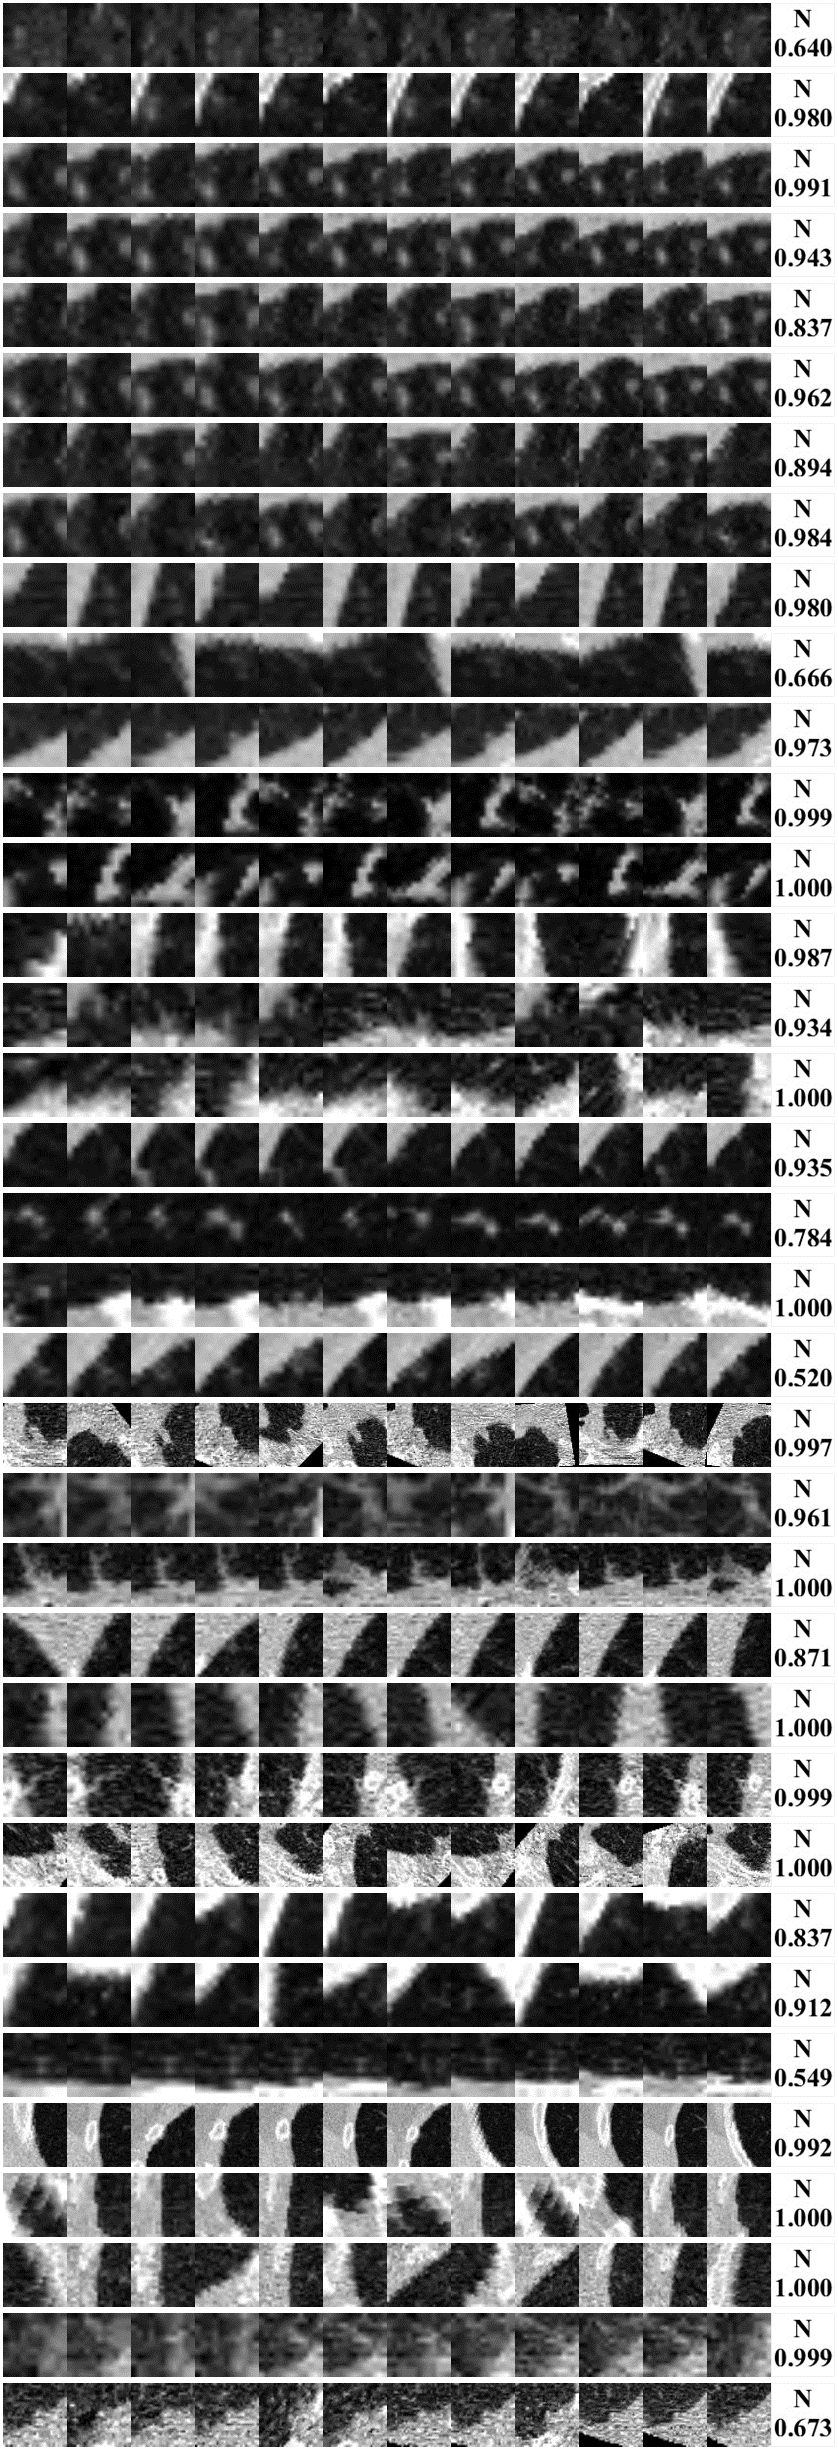
\includegraphics[width=0.45\columnwidth]{./images/elcap-msnodules-nonnodule1}
}
\end{figure}
\newpage
\begin{figure}[H]
\centering
\subfigure{
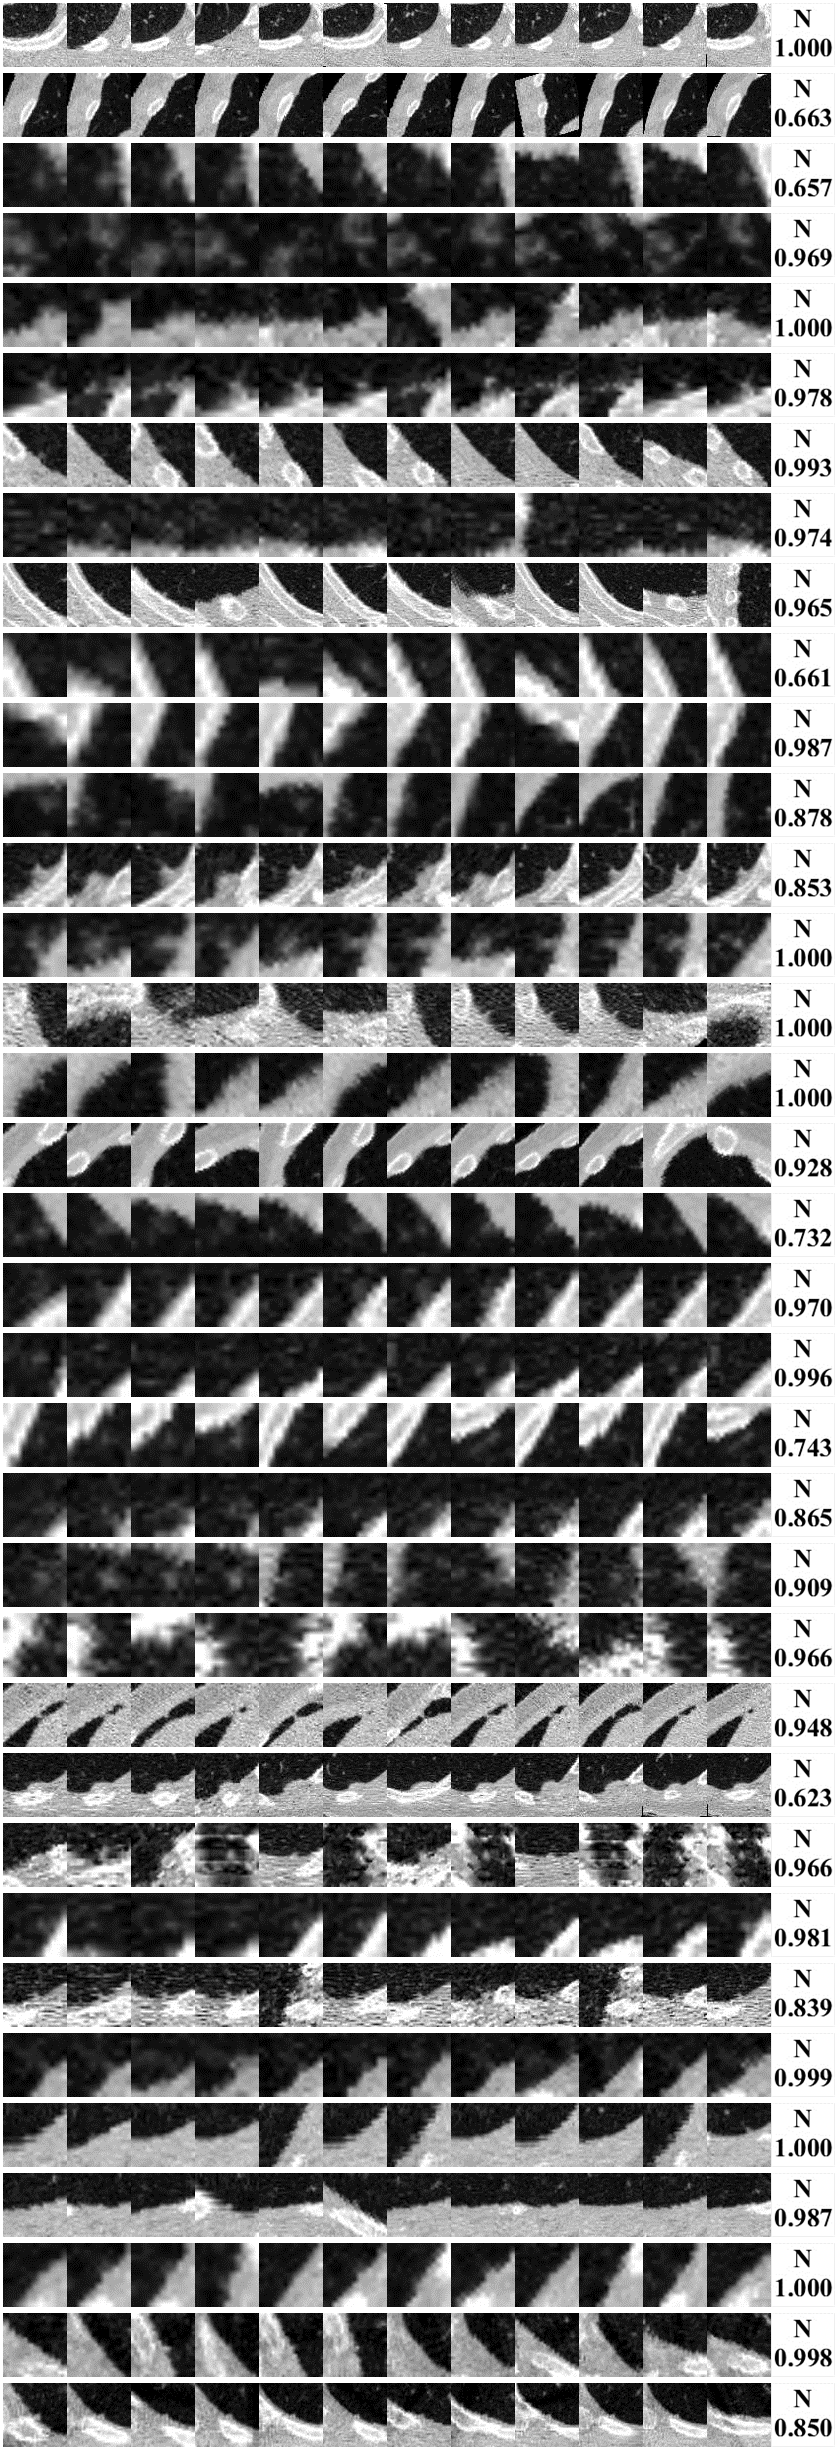
\includegraphics[width=0.45\columnwidth]{./images/elcap-msnodules-nonnodule2}
}
\hspace{.1in}
\subfigure{
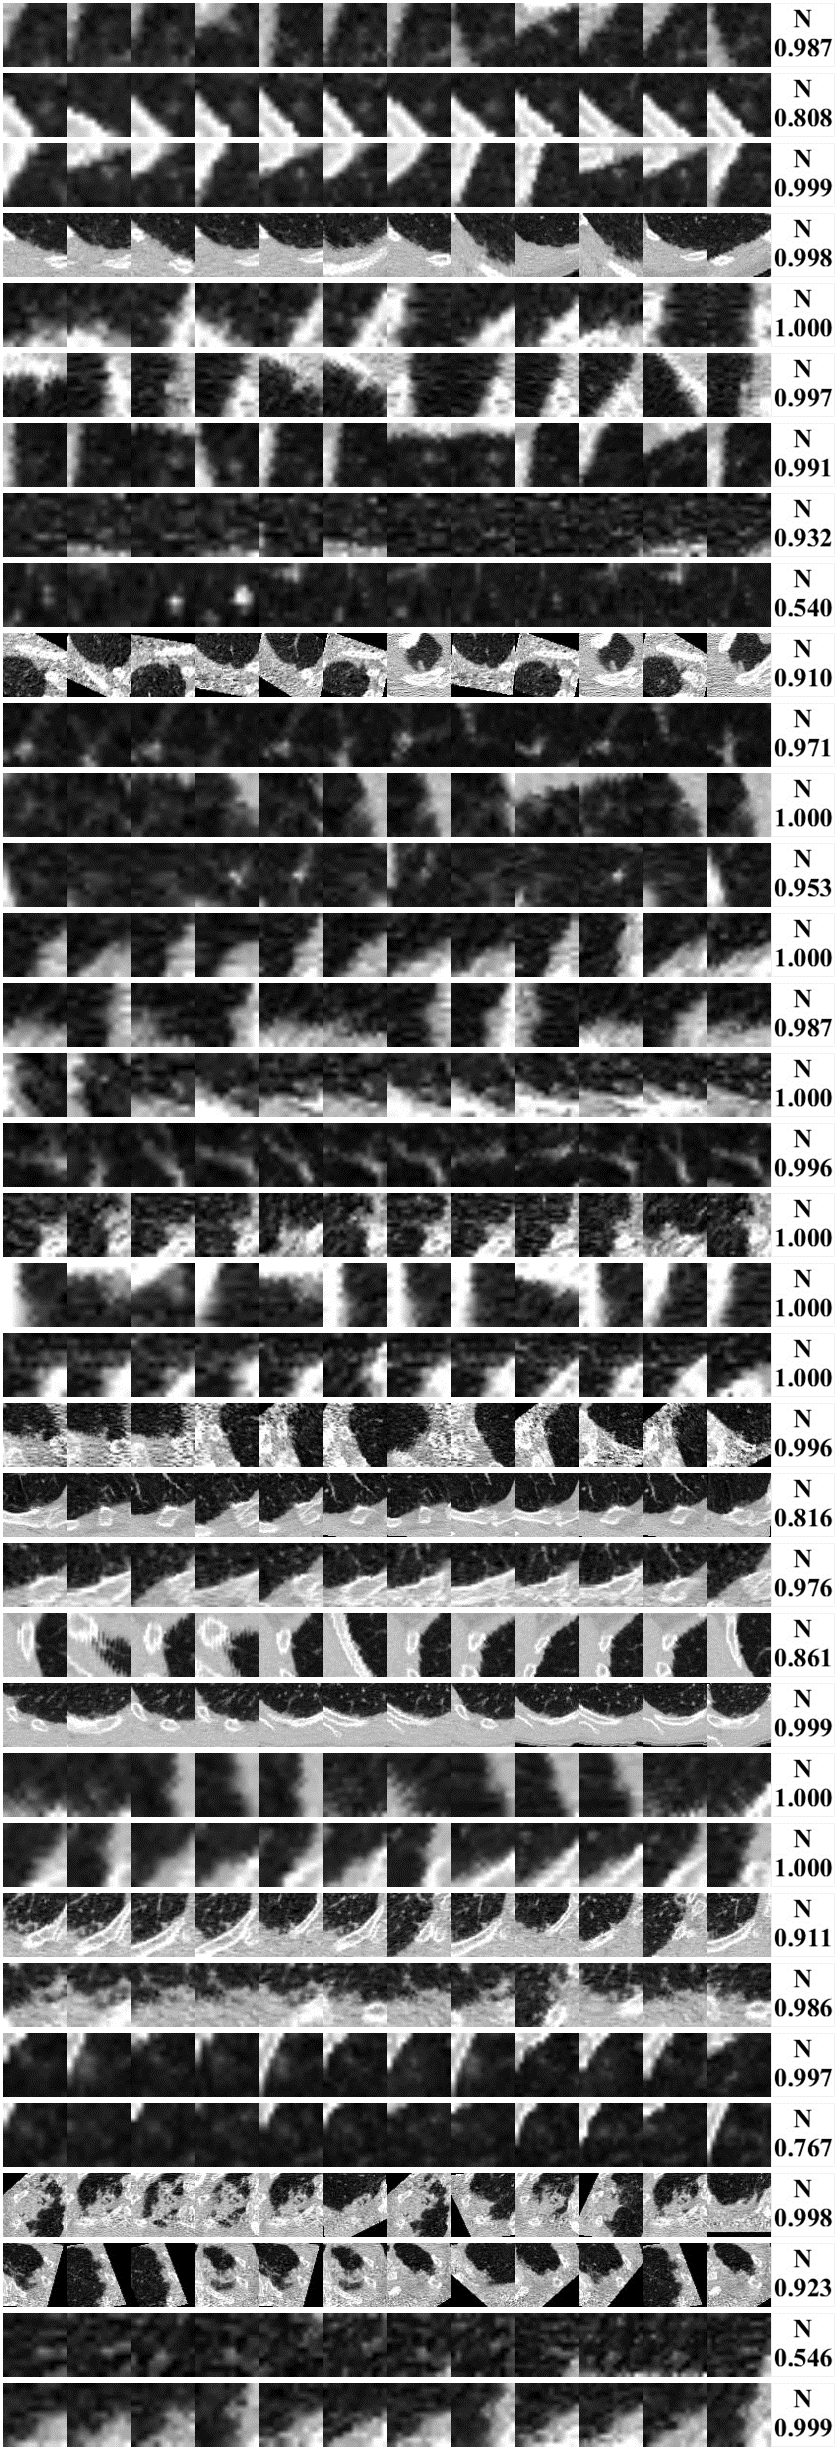
\includegraphics[width=0.45\columnwidth]{./images/elcap-msnodules-nonnodule3}
}
\end{figure}
\newpage
\begin{figure}[H]
\centering
\subfigure{
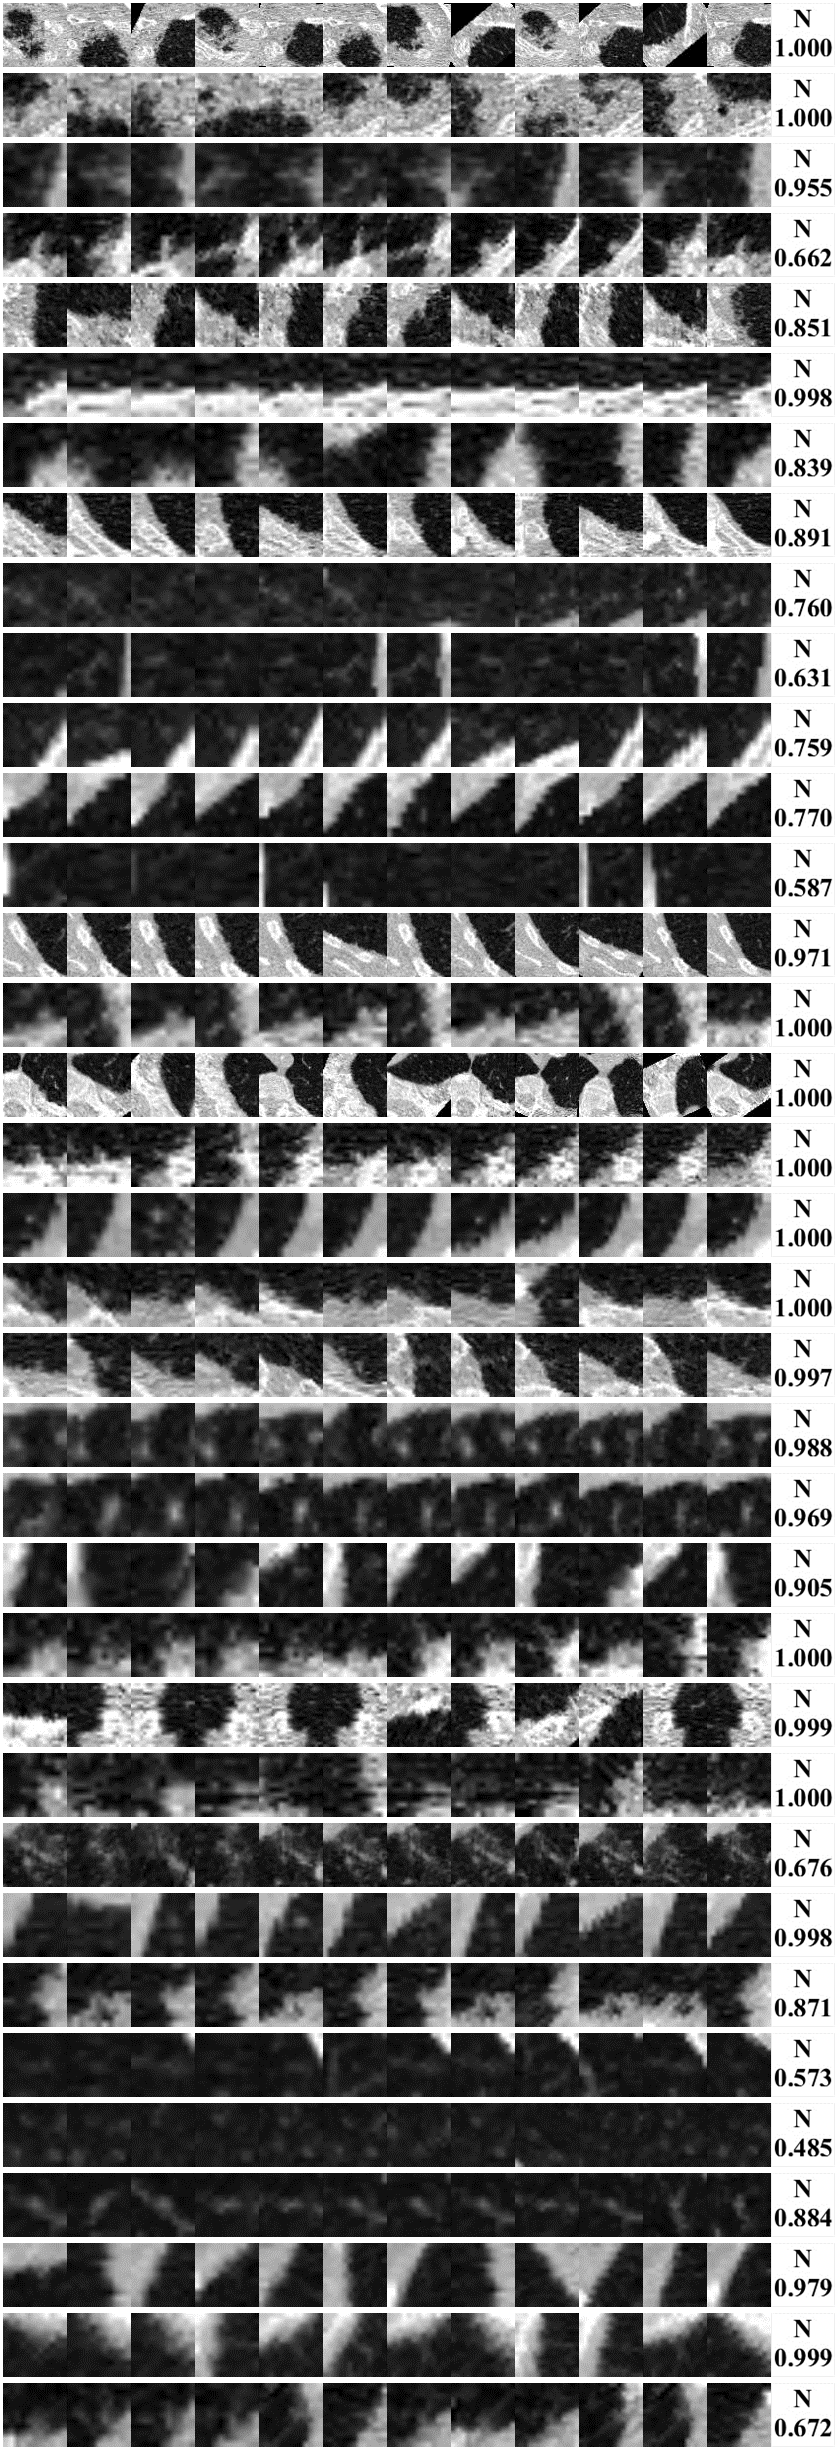
\includegraphics[width=0.45\columnwidth]{./images/elcap-msnodules-nonnodule4}
}
\hspace{.1in}
\subfigure{
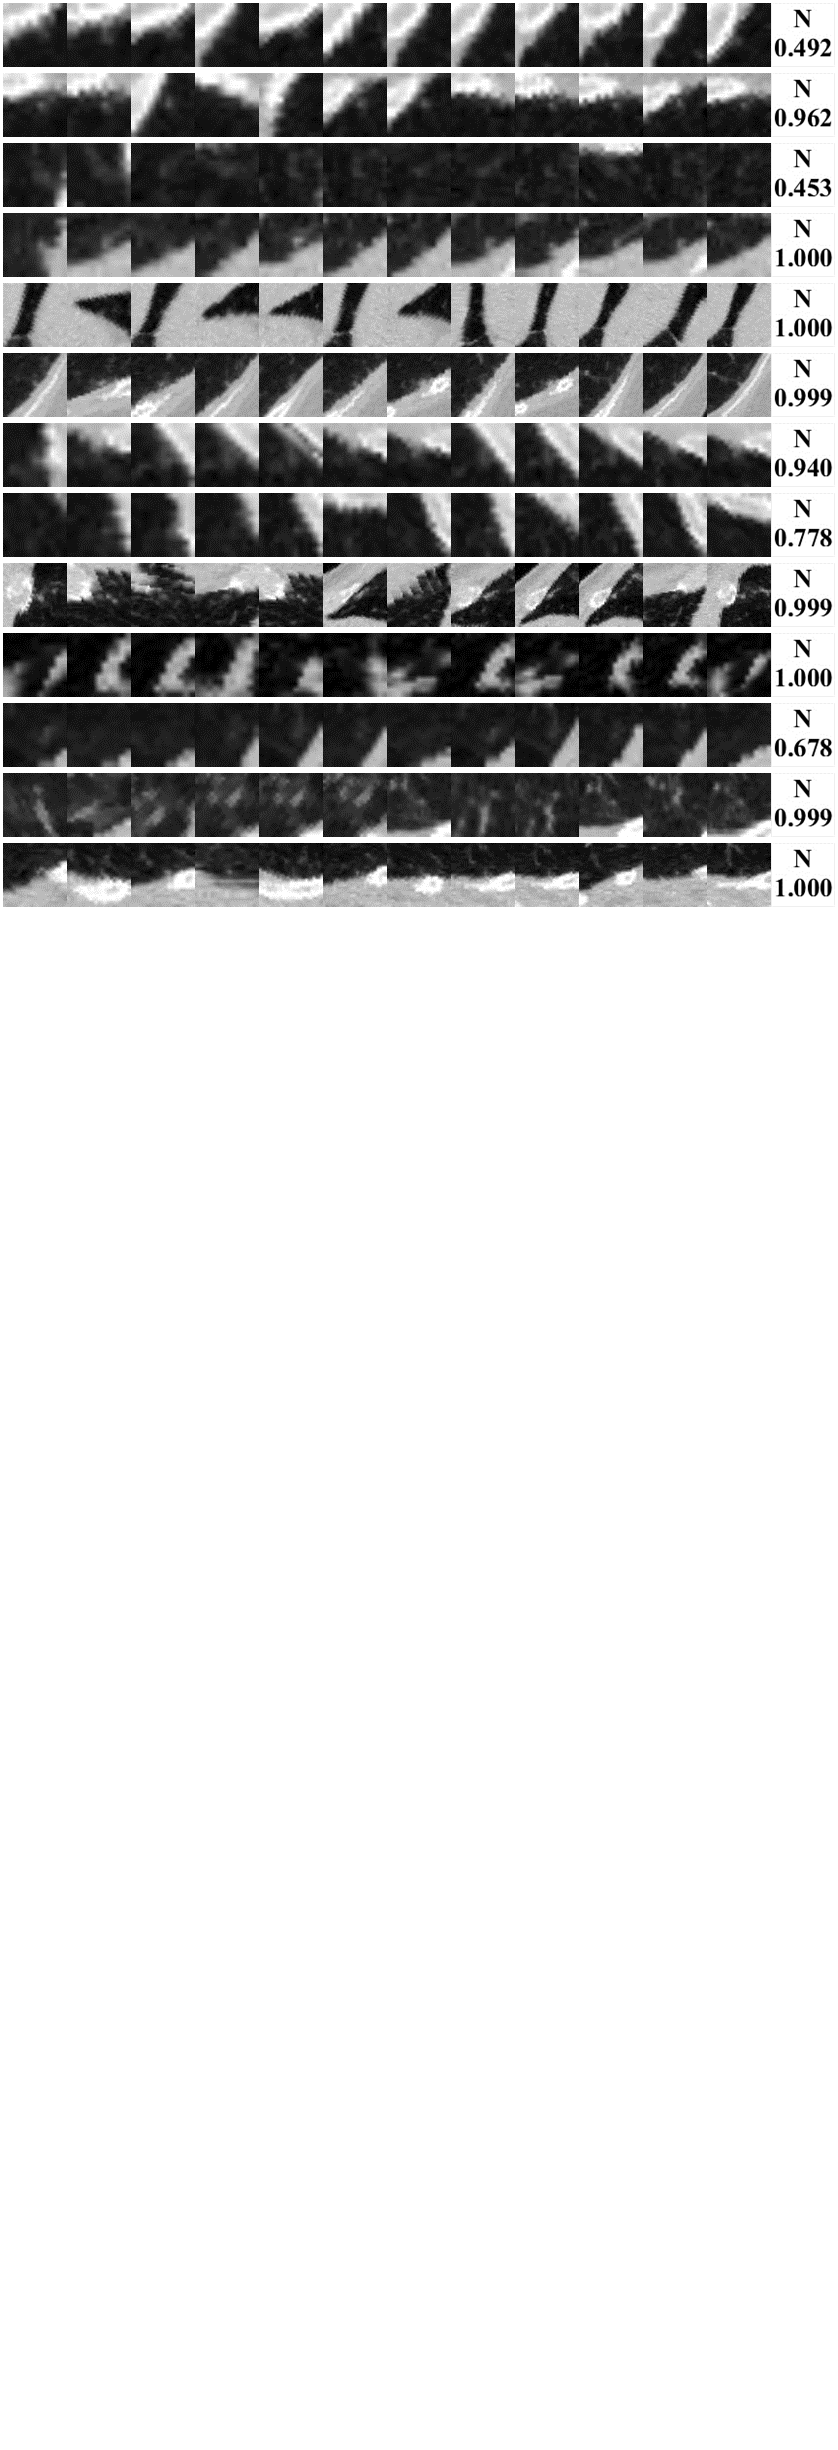
\includegraphics[width=0.45\columnwidth]{./images/elcap-msnodules-nonnodule5}
}
\end{figure}


\end{document}


